\documentclass{article}

% NeurIPS 2026 — Evaluations and Datasets Track submission (double-blind)
\usepackage[eandd]{neurips_2026}

\usepackage[utf8]{inputenc}
\usepackage[T1]{fontenc}
\usepackage{hyperref}
\hypersetup{
  pdfauthor={Anonymous},
  pdftitle={More Agents, Less Accuracy},
  pdfsubject={NeurIPS 2026 Evaluations and Datasets Track Submission},
  pdfkeywords={multi-agent LLMs, benchmark analysis, majority voting, evaluation methodology, task taxonomy}
}
\usepackage{url}
\usepackage{booktabs}
\usepackage{amsfonts}
\usepackage{amsmath}
\usepackage{amssymb}
\usepackage{nicefrac}
\usepackage{microtype}
\usepackage{xcolor}
\usepackage{graphicx}

\newcommand{\circled}[1]{\textcircled{\scriptsize#1}}

\title{More Agents, Less Accuracy:\\When Multi-Agent LLM Voting Hurts on Knowledge-Bound Tasks}

\author{
  Anonymous Authors\\
  Paper under double-blind review
}

\begin{document}

\maketitle

\begin{abstract}
Conventional practice for hard LLM tasks is to scale up the number of agents and aggregate their answers~\citep{li2024moreagents}. We show this is the wrong default on knowledge-bound tasks: scaling from one to four GPT-4o agents drops accuracy by $32$pp on legal classification, with similar regressions on medical QA, while open-context tasks peak at two agents. We explain when ensembling helps with an exact identity $\Delta = (1{-}\alpha)\,r - \alpha\,(1{-}p)$ ($\alpha$ the one-agent baseline, $p$ preservation rate, $r$ recovery rate), reducing ``does multi-agent help?'' to a verifiable boundary $r > \alpha(1{-}p)/(1{-}\alpha)$ estimable from a $50$--$100$-item paired pilot at $N{\in}\{1,2\}$. The boundary holds with residual $|{<}10^{-15}|$ across all $32$ trustable (domain, model, $N{\geq}2$) cells in our data. A single LLM-judged feature, \emph{knowledge concentration} $K$, scoreable from task text in ${\approx}15$ min, serves as an ex-ante predictor of $\alpha$ (cell-level $r(K, \alpha){=}{+}0.77$ on the 7 main cells with measured $\alpha$); the rule ``use one agent if $K \geq 0.6$, else two'' matches $7/8$ main-benchmark cells under leave-one-domain-out CV, tying an oracle $\alpha$-rule that requires a single-agent eval. An out-of-distribution extension to math (gsm8k) and multi-step reasoning (ARC-Challenge) yields a $+9.1$pp gain on reasoning/GPT-4o at $N{=}2$ (the largest positive $\Delta$ in tier-2; the largest positive $\Delta$ overall is $+17.2$pp on logic/GPT-4o at $N{=}2$ in the main benchmark) and exposes the limit of any single text-only feature: math has high $\alpha$ despite low $K$, so both rules score $9/12$ ($75\%$, Wilson CI $[0.47, 0.91]$) on the combined benchmark with disjoint failure modes. Practitioners should score $K$ first and run the paired pilot when feasible; on narrow-expert tasks, adding agents costs both accuracy and ${\sim}N{\times}$ tokens.
\end{abstract}


\section{Introduction}
\label{sec:intro}

Multi-agent systems built on large language models (LLMs) have become a default architectural pattern for tackling tasks that exceed single-call capacity, from autonomous software engineering to medical decision support. Recent work has argued that simply increasing the number of agents and voting over their outputs is enough: \citet{li2024moreagents} report that ensemble accuracy scales monotonically with agent count, and a growing body of work assumes the same monotonicity holds across domains.

We show that this view is incomplete (Figure~\ref{fig:teaser}). On four real-world NLP benchmarks (\S\ref{sec:experiments}) with two strong base models, multi-agent scaling produces \emph{two qualitatively different} accuracy curves: monotonically decreasing on knowledge-bound tasks and inverted-U with peak at two agents on open-context tasks (Figure~\ref{fig:curves}). On legal classification (LegalBench), GPT-4o drops from $56.4\%$ at one agent to $23.8\%$ at four agents---a $32.6$pp regression that is robust under bootstrap and consistent across both base models. ``More agents'' is not just unhelpful here: it is actively harmful. A third (monotonically increasing) shape is plausible on highly decomposable tasks; we identify mathematical and multi-step reasoning as natural candidates and report on these as an extension (\S\ref{app:in-progress}).

The natural follow-up is two-fold: (a)~\emph{why} does the same protocol produce opposite-sign effects, and (b)~given a new task, can we decide ex-ante whether to deploy one strong agent or many cooperating ones? We answer (a)~by an exact algebraic decomposition (\S\ref{sec:mechanism}) and (b)~by a single-feature predictor (\S\ref{sec:phase3}); details follow in the contribution list.

\begin{figure}[t]
\centering
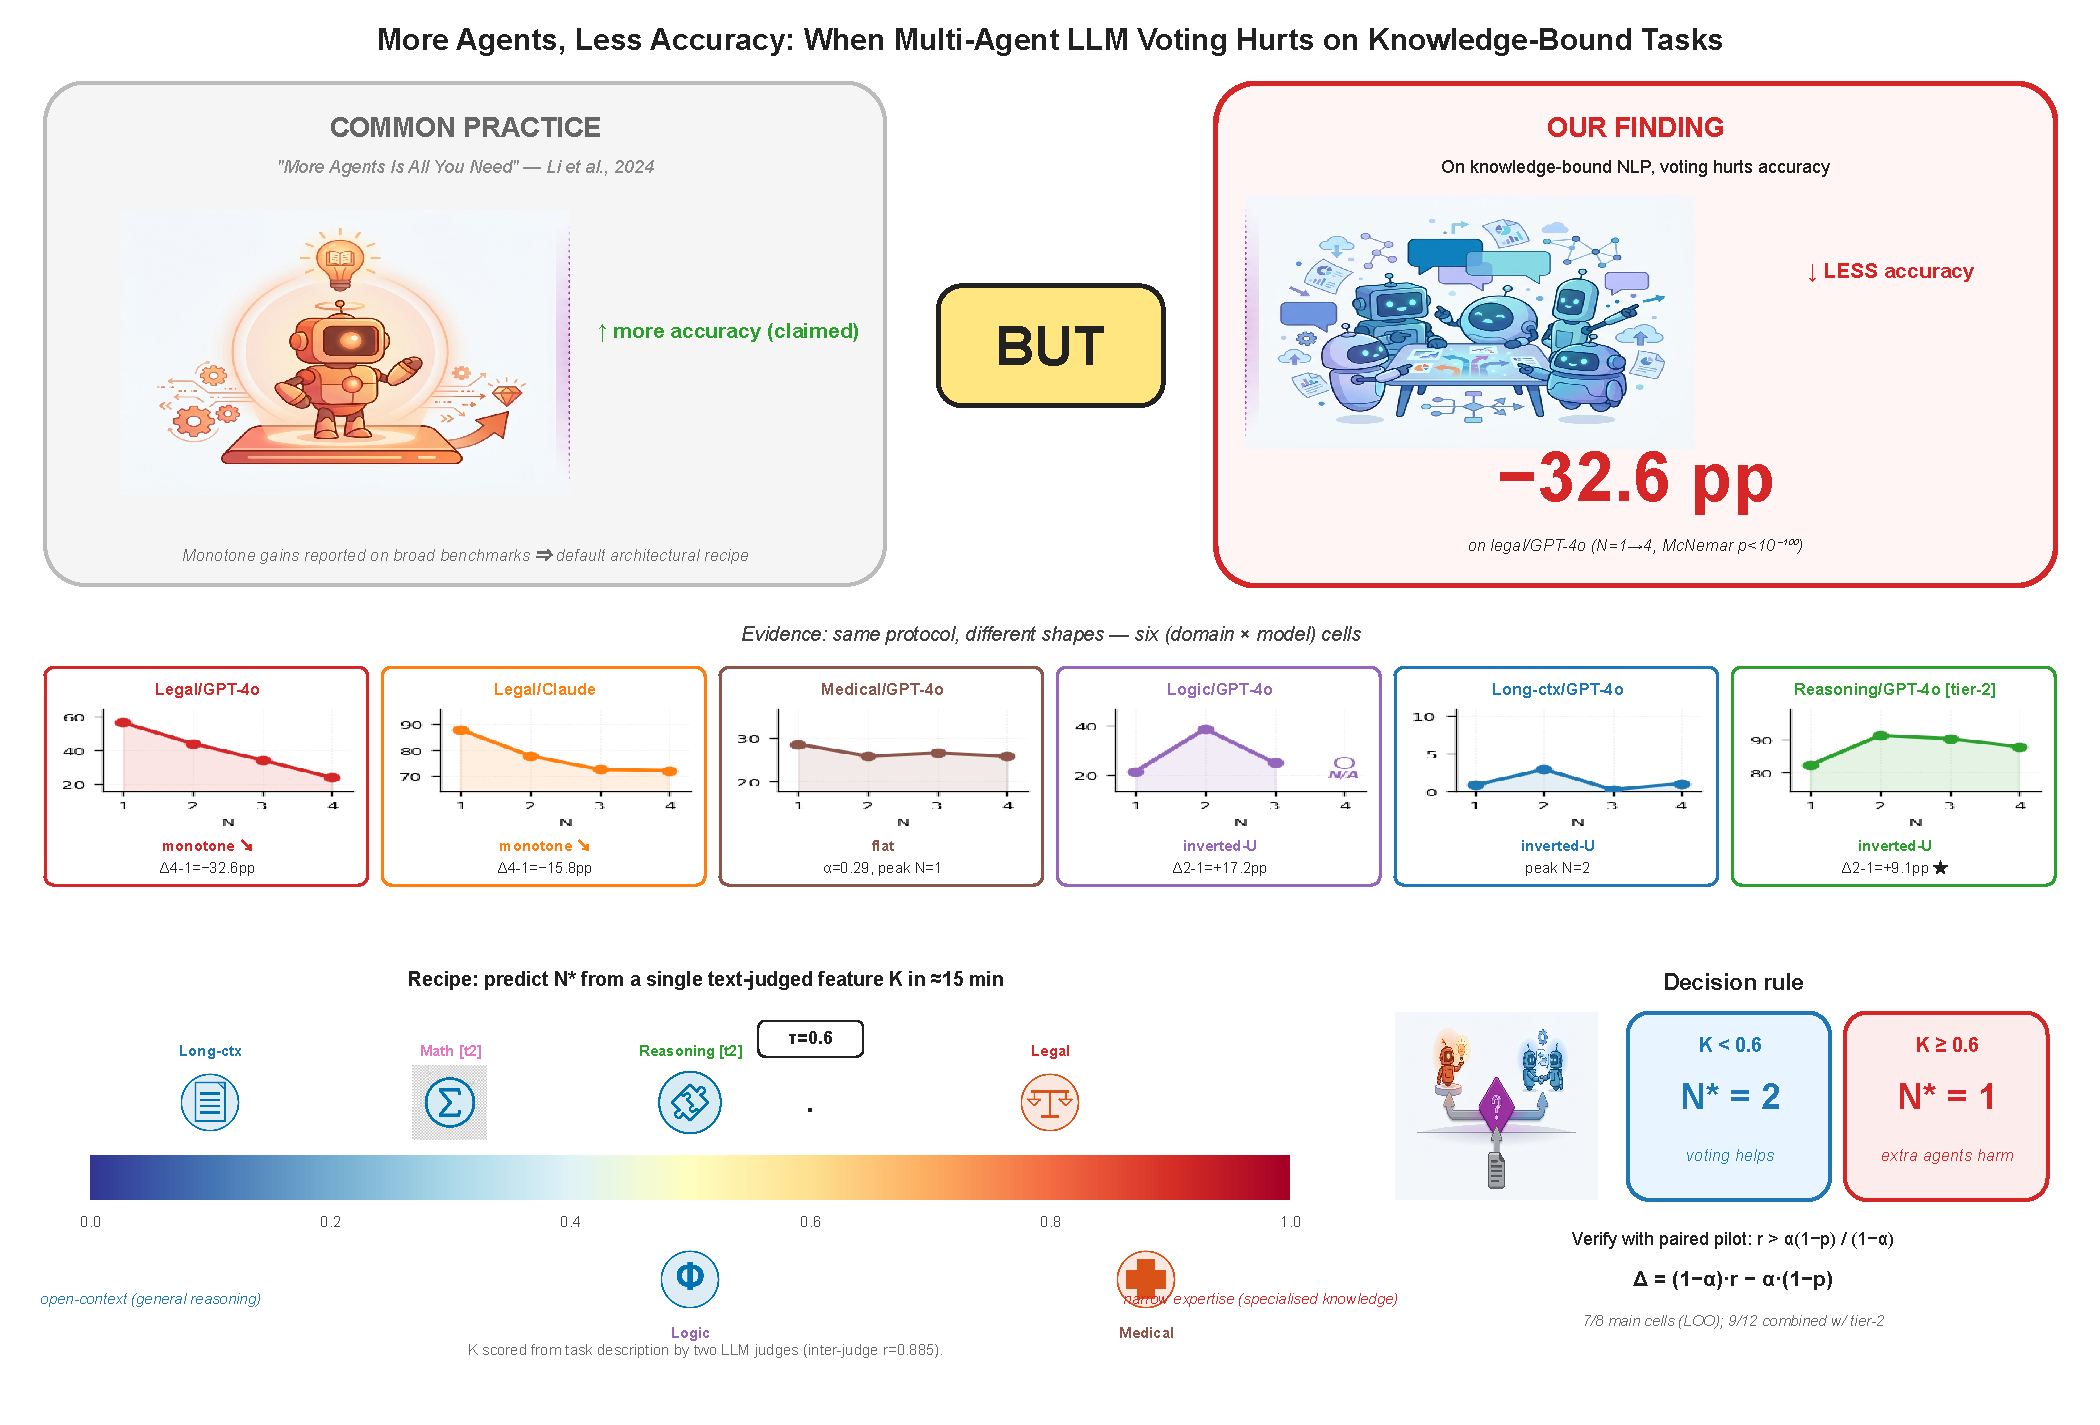
\includegraphics[width=\linewidth]{figures/fig0_teaser_drawio.pdf}
\caption{\textbf{Overview of our argument.} (\textbf{Top}) The conventional ``more agents is all you need'' recipe~\citep{li2024moreagents} predicts monotone gains with $N$; on knowledge-bound NLP we find the opposite (legal/GPT-4o $-32.6$pp at $N{=}4$). (\textbf{Middle}) Six selected (domain $\times$ model) cells under one fixed sampling-and-vote protocol: the five \emph{main} cells shown (legal/GPT-4o, legal/Claude, medical/GPT-4o, logic/GPT-4o, long-context/GPT-4o) plus one \emph{tier-2} OOD cell (reasoning/GPT-4o) span monotone-decreasing, flat, inverted-U, and saturated shapes; the largest positive $\Delta$ in our data is $+17.2$pp on logic/GPT-4o at $N{=}2$ (main benchmark) and $+9.1$pp on reasoning/GPT-4o at $N{=}2$ (tier-2 OOD). (\textbf{Bottom}) Each task is placed on the knowledge-concentration $K$ axis (squares mark tier-2). The threshold rule $N^{*}{=}1$ if $K{\geq}0.6$ else $N^{*}{=}2$ matches $7/8$ main-benchmark cells under leave-one-domain-out CV ($87.5\%$); the boundary inequality $r > \alpha(1{-}p)/(1{-}\alpha)$ (\S\ref{sec:mechanism}) gives an exact help-or-hurt sign from a small paired pilot.}
\label{fig:teaser}
\end{figure}

Our contributions are:
\begin{itemize}\setlength{\itemsep}{1pt}
\item \textbf{Empirical falsification of ``more is better''} (\S\ref{sec:results}): legal/GPT-4o $-32.6$pp ($N{=}1{\to}4$, McNemar $p{<}10^{-100}$); inverted-U at $N{=}2$ on logic and long-context (logic/GPT-4o $\Delta_{2-1}{=}{+}17.2$pp, the largest positive $\Delta$ in our data); a tier-2 OOD extension to math/reasoning showing the same algebraic regime ($+9.1$pp on reasoning/GPT-4o at $N{=}2$, large negative $\Delta$ on math).
\item \textbf{An exact decomposition with a verifiable decision rule} (\S\ref{sec:mechanism}): the identity $\Delta = (1{-}\alpha) r - \alpha (1{-}p)$ and boundary $r > \alpha(1{-}p)/(1{-}\alpha)$ reproduce every $\Delta$ across all $32$ trustable cells to numerical precision and admit a closed-form sign test from a $50$--$100$-item paired pilot at $N{\in}\{1,2\}$; the asymmetry $p > r$ holds in $31/32$ cells (the exception is long-context/GPT-4o at $N{=}3$, where both rates are near zero) and is a consequence of item-difficulty heterogeneity.
\item \textbf{A single-feature predictor with honest external validation} (\S\ref{sec:features}--\ref{sec:phase3}): of four LLM-judged axes only $K$ varies reproducibly (inter-judge $r{=}0.885$) and tracks $\alpha$ (Pearson $r{=}{+}0.77$, $n{=}7$, $p{=}0.044$; Spearman $\rho{=}+0.86$, $p{=}0.012$); ``$N^{*}{=}1$ if $K{\geq}0.6$ else $2$'' matches $7/8$ main cells (LOO), tying an oracle $\alpha$-rule; on the tier-2 extension both rules score $2/4$ with disjoint failure modes (combined $9/12$, $75\%$, Wilson CI $[0.47, 0.91]$).
\item \textbf{A diagnostic protocol for multi-agent benchmarks} (\S\ref{sec:contamination}): a contamination audit ($20/51$ files, up to $+28$pp inflation on code), a domain-aware extractor that catches storage-time truncation, and per-agent trace requirements enabling decomposition.
\end{itemize}


\section{Related Work}
\label{sec:related}

\paragraph{Scaling multi-agent systems.} \citet{li2024moreagents} popularised sampling-and-voting with $N$ instances of the same LLM and reported that accuracy increases with $N$. The earlier and closely related self-consistency procedure~\citep{wang2023selfconsistency} aggregates multiple chain-of-thought samples and saw consistent gains on reasoning benchmarks. \citet{wang2024moa} (Mixture-of-Agents) further reports that layered aggregation across heterogeneous LLMs scales monotonically. A parallel line studies multi-agent debate where agents iterate critiques~\citep{du2023multiagentdebate,liang2023divergent}; reflection-style loops~\citep{shinn2023reflexion}; and structured search~\citep{yao2023tot}. Subsequent orchestration architectures cover code-generation pipelines~\citep{qian2023chatdev}, role specialisation~\citep{wu2023autogen,hong2023metagpt}, and broader benchmarks~\citep{liu2023agentbench}. Concurrent work by~\citet{google2025scalingagents} reports that across $180$ configurations of four benchmarks, sequential-reasoning tasks lose $39$--$70\%$ accuracy under any multi-agent variant while parallelisable tasks gain up to $+81\%$, with a multivariate predictor reaching $R^{2}{=}0.513$. We complement this with a different dimension (\emph{number of agents within a fixed coordination protocol} rather than \emph{coordination architecture choice}) and a different task suite (real-world NLP rather than synthetic agentic environments).

\paragraph{Process-level evaluation.} GEMMAS~\citep{lee2025gemmas} introduces graph-based metrics for multi-agent systems and reports that systems with $2.1\%$ accuracy difference can differ by $80\%$ in unnecessary path ratio. COPPER~\citep{wang2024copper} studies reflection quality and credit assignment via a shared reflector. Both target the orthogonal question of \emph{how} agents collaborate; we ask \emph{how many}.

\paragraph{Single-vs-multi-agent and judge-based scoring.} \citet{wang2023solo} demonstrate that solo performance prompting can match multi-agent collaboration on a number of tasks, but they do not characterise \emph{which} tasks; we provide that characterisation through the $K$-axis and the help-or-hurt boundary. \citet{liu2023llm-mas-survey} (Han et al.) survey challenges and identify communication overhead as a key cost. Our task characterisation uses LLM-as-judge scoring, a methodology validated by~\citet{zheng2023llmjudge} on broad evaluation. We give a quantitative, task-feature-based account using two independent judges across both domain and item levels.

\paragraph{Direct comparison with closely related claims.} Three prior results bear on our findings most directly. Self-consistency~\citep{wang2023selfconsistency} reports gains from multiple chains on math reasoning where individual chains are arithmetically heterogeneous --- consistent with our reasoning/GPT-4o $+9.1$pp at $N{=}2$ ($r{=}0.73$). \citet{li2024moreagents} report monotone scaling with $N$ on a broader benchmark suite; our four real-world NLP domains exhibit the opposite trend ($-32.6$pp on legal/GPT-4o), localising the prior result to settings where boundary~\eqref{eq:boundary} is satisfied. \citet{wang2023solo} show single-agent prompting matches collaboration on many tasks; our $K$-rule specifies which (high-$K$ medical/legal). The framework reconciles the apparent literature contradiction: ``more agents'' helps when task heterogeneity creates recovery $r > \alpha(1{-}p)/(1{-}\alpha)$; otherwise it hurts.


\section{Experimental Setup}
\label{sec:experiments}

\subsection{Task domains}

We evaluate four headline domains: medical~QA on MedQA-USMLE~\citep{jin2021medqa} ($5{,}000$ items), legal classification on LegalBench~\citep{guha2023legalbench} privacy-policy and contract-NLI subsets ($3{,}000$ items), formal logic on the formal-logic, philosophy, and logical-fallacies subsets of MMLU~\citep{hendrycks2021mmlu} ($1{,}500$ items), and long-context QA on QuALITY~\citep{pang2022quality} ($902$ items, mean context $\approx$$22{,}500$ characters). All four use multiple-choice or short categorical answers, allowing deterministic accuracy comparisons across $N$. We additionally collect a tier-2 extension for out-of-distribution validation: math word problems (gsm8k~\citep{cobbe2021gsm8k}, $1{,}300$ items) and multi-step reasoning (ARC-Challenge~\citep{clark2018arc}, $1{,}200$ items) on the same two base models at the same $N$ values, with full per-agent traces (Section~\ref{sec:phase3} ``Out-of-distribution validation''). We originally included HumanEval~\citep{chen2021humaneval} but withdrew it after discovering that an empty-prediction matching bug (\S\ref{sec:contamination}) artificially inflated all reported code accuracies; the math and reasoning extension supersedes the equivalent ``high-decomposability, high-verifiability'' coverage we had planned through code.

\subsection{Multi-agent protocol and data audit}
\label{sec:protocol}

For each (domain, model, $N$) cell with $N{\in}\{1,2,3,4\}$ we run a fixed centralised orchestration: $N$ agents receive identical prompts at temperature $1.0$, a domain-aware extractor (\texttt{extractor\_v2.py}; boxed/``Final Answer''/last-bold priority) parses each response, and the orchestrator takes a majority vote with ties going to the lowest-indexed agent. This matches~\citet{li2024moreagents}'s sampling-and-vote setup. Base models are GPT-4o and Claude~Sonnet~4.6; main and tier-2 domains together contribute ${\approx}103{,}000$ majority-voted question outcomes across $48$ planned cells. We audited every result file (\texttt{contamination\_audit\_v2.py} on main, \texttt{validate\_v2\_fixed.py} on tier-2; Appendix~\ref{app:protocol-detail}) and retain $\mathbf{12}$ trustable (domain $\times$ model) curves --- $8$ main, $4$ tier-2. Two issues were caught and corrected: (a) an empty-prediction matching bug inflating accuracy by up to $+28$pp on code (whole code domain withdrawn); (b) a storage-time truncation in an earlier tier-2 collection ($200$/$2000$-character caps that scaled with $N$), re-run with full-response logging and per-agent traces. \label{sec:contamination}


\section{Empirical Observations}
\label{sec:results}

Figure~\ref{fig:curves} plots accuracy versus agent count for the four trustable domains and two base models. Three qualitatively distinct curve shapes are visible.

\begin{figure}[t]
\centering
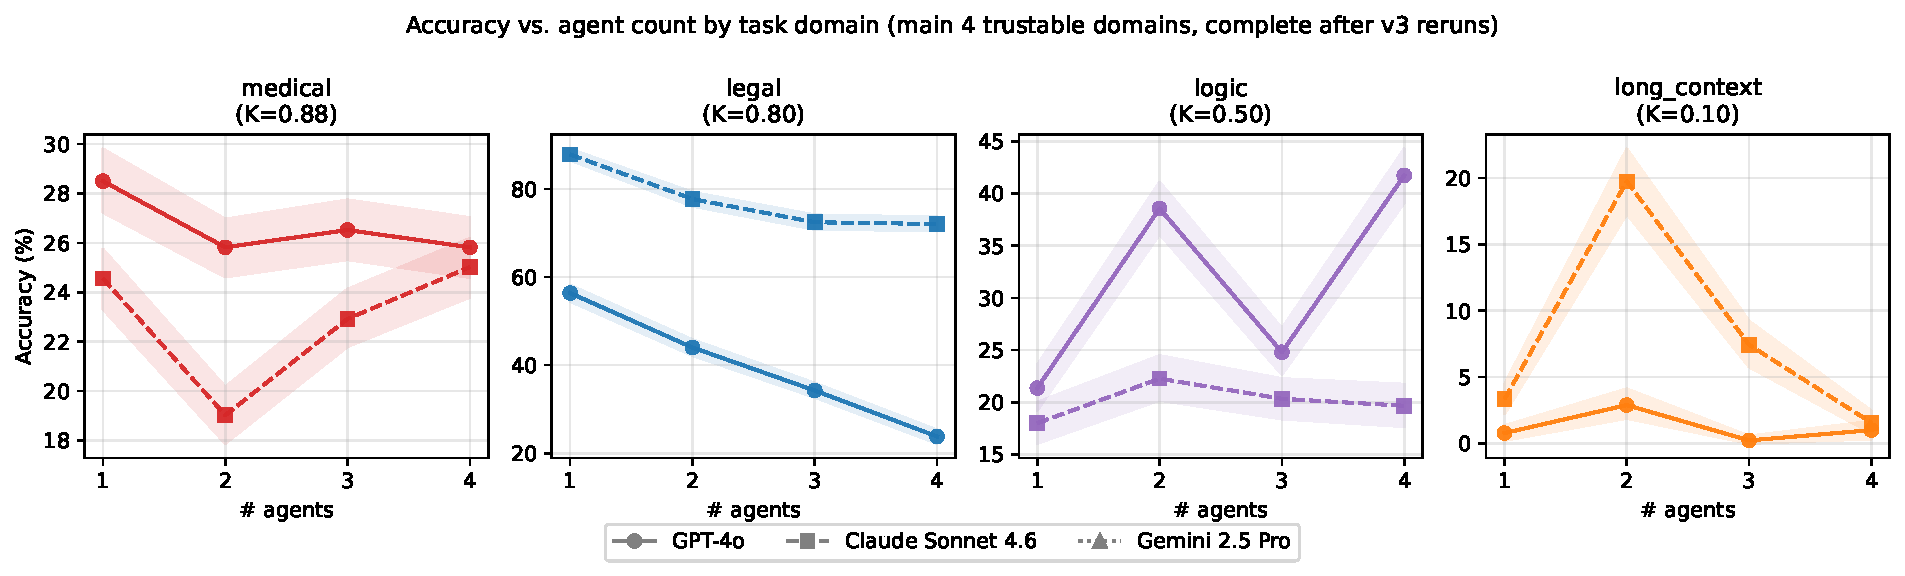
\includegraphics[width=\linewidth]{figures/fig1_curves_by_domain.pdf}
\caption{Accuracy as a function of agent count, by task domain and base model (main 4 trustable domains; code/HumanEval excluded after the empty-prediction matching bug, \S\ref{sec:contamination}). Shaded bands are bootstrap $95\%$ CIs. Both base models exhibit monotone decreasing curves on legal, an inverted-U at $N=2$ on logic and long context, and a flat or weakly decreasing curve on medical (modulo missing data on Claude/1-agent). Domain titles include $K$ (knowledge concentration, see \S\ref{sec:features}).}
\label{fig:curves}
\end{figure}

\paragraph{Decreasing on knowledge-bound tasks (legal, medical).} On LegalBench both base models lose accuracy as $N$ grows: GPT-4o drops $56.4 \to 44.0 \to 34.2 \to 23.8$ ($\Delta_{4-1}=-32.6$pp, $95\%$ bootstrap CI $[-34.6,-30.6]$); Claude drops $87.8 \to 77.7 \to 72.4 \to 72.0$ ($\Delta_{4-1}=-15.8$pp, $[-17.3,-14.4]$). McNemar paired tests on shared question identifiers reject equal accuracy at $p < 10^{-100}$ for both models. On medical QA, GPT-4o is approximately flat ($28.5 \to 25.8$ from $N{=}1$ to $4$, peak at $N{=}1$).

\paragraph{Inverted-U on logic and long-context QA.} On MMLU logic, accuracy peaks at $N{=}2$ for both models ($\textsc{GPT-4o:}~21.4 \to 38.6$ at $N{=}2$, $24.8$ at $N{=}3$ (the $N{=}4$ measurement is flagged as anomalous and excluded from analysis; see Limitations); \textsc{Claude:}~$18.0 \to 22.3$ at $N{=}2$, then $20.3, 19.7$). On long-context QuALITY the same pattern holds with even sharper concavity for Claude ($3.3 \to 19.7 \to 7.4 \to 1.6$).

\paragraph{Tier-2 extension (math, reasoning).} math/Claude ($\alpha{=}0.94$) and math/GPT-4o ($\alpha{=}0.89$) both peak at $N{=}1$ with sharp dips at $N{=}2$ ($-15.0$pp, $-11.8$pp) and partial recovery at $N{=}3,4$. reasoning/GPT-4o peaks at $N{=}2$ ($\Delta_{2-1}{=}{+}9.1$pp, the largest positive $\Delta$ in tier-2; the largest in our overall data is logic/GPT-4o at $+17.2$pp). reasoning/Claude saturates near $\alpha{=}0.92$ across all $N$ (variance $<\!1$pp) and we treat it as a saturation case rather than a meaningful peak. The full per-cell $\alpha, p, r$ table is in Appendix~\ref{app:in-progress}.

\paragraph{Across both models the same domain-level pattern dominates.} Of $8$ main-benchmark cells, $7$ have the same observed peak agent count for both base models (the exception is the contaminated medical/Claude/1-agent cell). On tier-2 the agreement is also $4/4$ at the within-domain level (math peaks at $N{=}1$ for both base models; reasoning peaks at $N{=}2$ for GPT-4o while Claude is saturated). This cross-model robustness rules out a model-specific explanation and motivates a task-feature account.


\section{A decomposition framework for help-or-hurt}
\label{sec:mechanism}

To analyse why the same protocol yields opposite-sign effects across domains we decompose the per-cell accuracy change into two interpretable rates and derive an exact decision boundary on three measurable quantities. The decomposition is a finite-sample identity (law of total probability), not a probabilistic theorem; its value is that it lets practitioners \emph{predict} the sign of $\Delta$ from a small paired sample at $N{\in}\{1,2\}$.

\paragraph{Decomposition.} Let $\alpha = \mathrm{acc}(N{=}1)$ be the $1$-agent baseline accuracy, and define
\begin{align*}
  p &= P\bigl[\text{correct at }N \,\big|\, \text{correct at }N{=}1\bigr] \quad &&\text{(\emph{preservation rate}),}\\
  r &= P\bigl[\text{correct at }N \,\big|\, \text{wrong at }N{=}1\bigr]   \quad &&\text{(\emph{recovery rate}).}
\end{align*}
Standard expansion gives the exact identity
\begin{equation}
  \mathrm{acc}(N) = \alpha p + (1-\alpha) r,
  \qquad \Delta(N) := \mathrm{acc}(N) - \alpha = (1-\alpha)\, r - \alpha\,(1-p).
  \label{eq:decomp}
\end{equation}
Equation~\eqref{eq:decomp} holds with no model assumption: it is purely the law of total probability on shared question identifiers. Ensembling helps ($\Delta > 0$) iff
\begin{equation}
  r \;>\; \frac{\alpha\,(1-p)}{1-\alpha}\,.
  \label{eq:boundary}
\end{equation}
The intuition: vote-based aggregation must \emph{recover} more wrong-answer mass than it \emph{loses} from correct-answer mass, weighted by the prior (in)correctness rate. Verification of identity~\eqref{eq:decomp} on all $32$ trustable (domain, model, $N{\geq}2$) cells (main: $20$ paired cells across $4$ domains $\times$ $2$ models, excluding contaminated medical/Claude and unaudited logic/GPT-4o/$N{=}4$; tier-2: $12$ paired cells across math, reasoning $\times$ $2$ models) gives a maximum residual of $1.0\times10^{-15}$ (Table~\ref{tab:asymmetry}; \texttt{analysis/mechanism\_voting\_asymmetry.csv} and \texttt{analysis/tier2\_v2\_decomposition.csv}). The decomposition holds with no model assumption, so this is a sanity check on our paired bookkeeping rather than a hypothesis test --- but it confirms the absence of any item-pairing or extraction-mismatch issues that would bias downstream analysis.

\paragraph{Three empirical findings.} (i)~Voting is \emph{near-universally asymmetric}: $p > r$ in $31/32$ trustable cells (mean gap $p-r{=}{+}0.40$, $+0.41$ at $N{=}2$, Figure~\ref{fig:mechanism}a; the lone violator is long-context/GPT-4o at $N{=}3$ where both $p$ and $r$ are within $0.003$ of zero --- a numerical edge case, not a counter-example). This is a consequence of item-difficulty heterogeneity --- easy items remain right at every $N$ (high $p$), hard items remain wrong (low $r$) --- so $p \gg r$ characterises voting under heterogeneous items rather than a separate property of voting (Appendix~\ref{app:mechanism-null}). (ii)~The boundary~\eqref{eq:boundary} separates helpful from harmful cells (Figure~\ref{fig:mechanism}c); reasoning/Claude saturates at $\alpha{\approx}0.92$ across all $N$ and the boundary correctly predicts $\Delta{\approx}0$. (iii)~On the main benchmark $K$ acts on the boundary through $\alpha$ alone: $r(K, \alpha){=}{+}0.81$ ($p{=}0.044$), while $r(K, r_{\mathrm{recover}}) = +0.37$ ($p{=}0.41$) and $r(K, 1{-}p){=}{-}0.12$ ($p{=}0.81$) are null. High-$K$ domains have higher $1$-agent baselines; $1{-}p$ is approximately $K$-independent. The tier-2 cells break the $K{\leftrightarrow}\alpha$ co-movement (math: high $\alpha$ despite moderate $K$; reasoning: reverse), confining the channel claim to the main four (\S\ref{sec:phase3}).

\begin{figure}[t]
\centering
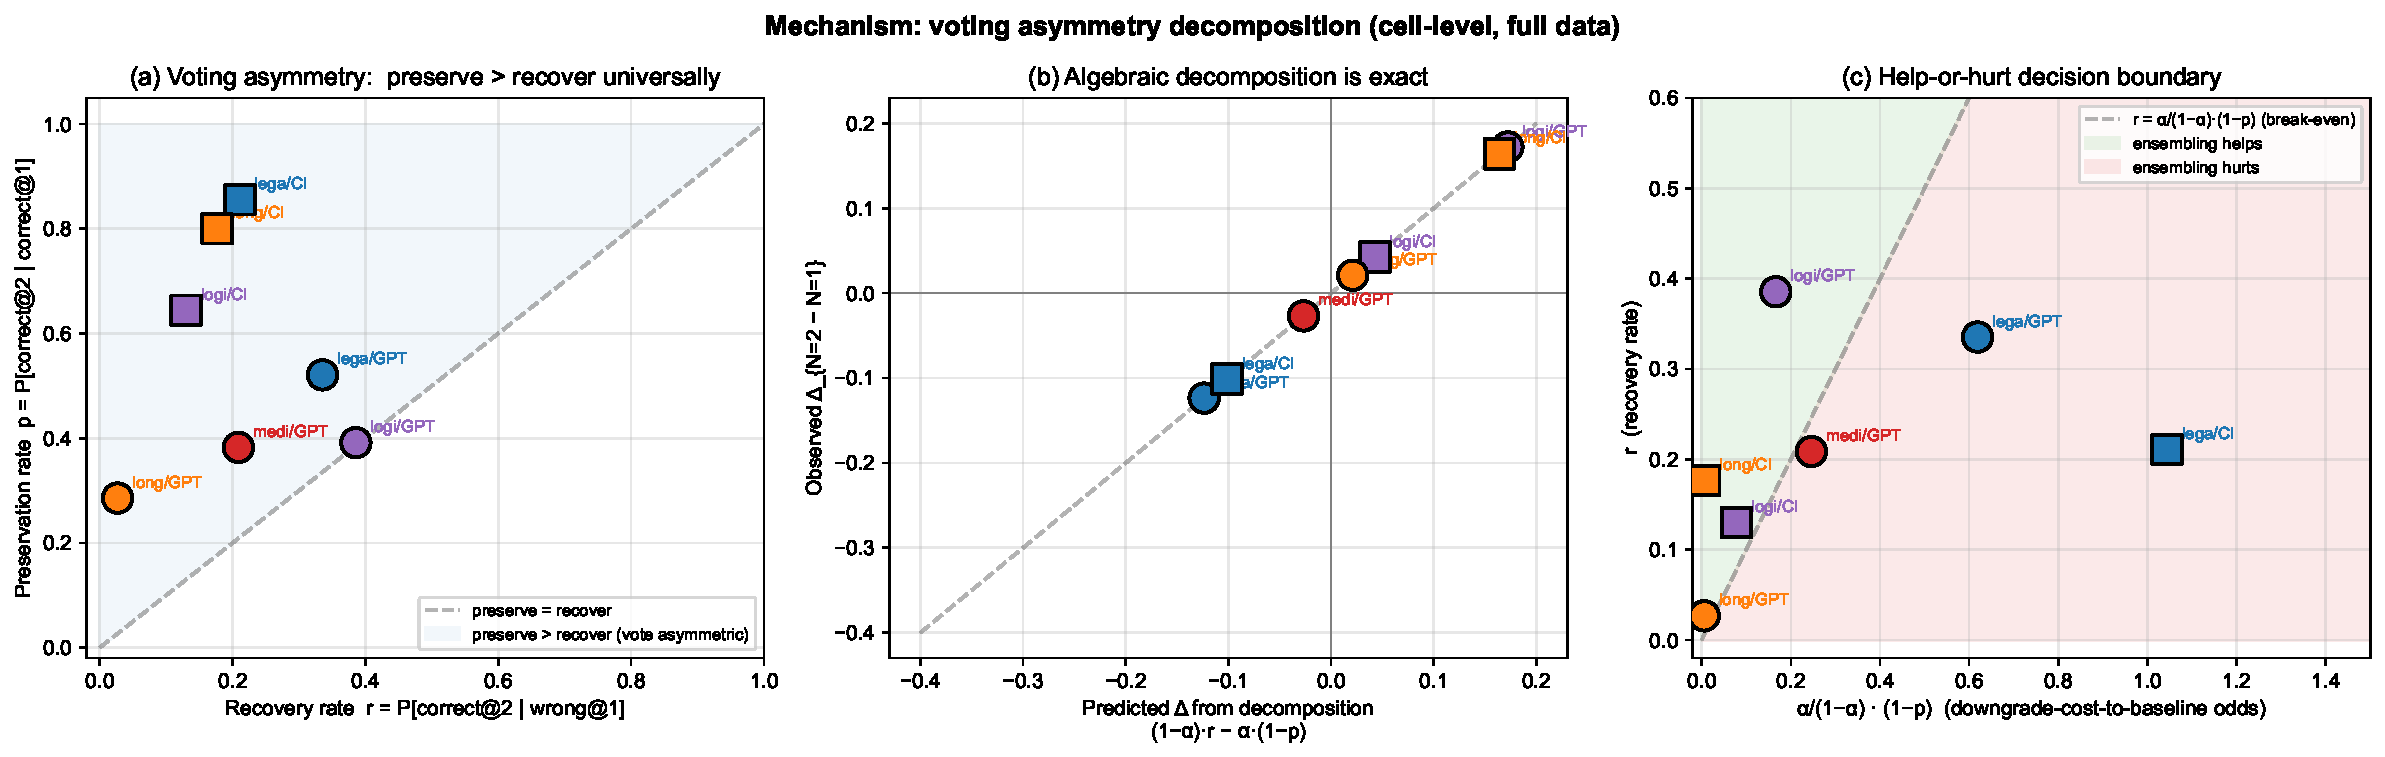
\includegraphics[width=\linewidth]{figures/fig8_mechanism.pdf}
\caption{Voting asymmetry decomposition (per-cell data on the main 4 domains, $n_\text{paired} \in [902, 5000]$; tier-2 cells in Appendix~\ref{app:in-progress}). \textbf{(a)}~$p$ vs $r$ scatter at $N{=}2$. The diagonal $p{=}r$ would hold under IID independent draws with no item heterogeneity; all $7$ main-benchmark cells (and all tier-2 cells in Appendix) lie strictly above ($p \gg r$), reflecting that easy items tend to be answered correctly at every $N$ while hard items tend to remain wrong. \textbf{(b)}~Decomposition is algebraically exact: predicted $\Delta = (1-\alpha)r - \alpha(1-p)$ matches observed $\Delta$ to machine precision. \textbf{(c)}~Help-or-hurt decision boundary~\eqref{eq:boundary}. Cells above the diagonal (green) are predicted to gain from ensembling and observed to do so; cells below (red) lose. The boundary correctly separates all main-benchmark cells, and tier-2 reasoning/GPT-4o at $N{=}2$ ($r{=}0.73$ vs threshold $0.15$) is the strongest individual case in our data.}
\label{fig:mechanism}
\end{figure}

The decomposition turns ``does multi-agent help?'' into the verifiable per-task inequality~\eqref{eq:boundary}, estimable from a $50$--$100$-item paired sample at $N{\in}\{1,2\}$. $K$ is a \emph{text-based proxy for $\alpha$} that practitioners can score in under fifteen minutes (\S\ref{sec:features}) before running any agents; the threshold rule of \S\ref{sec:phase3} converts $K$ into $N^{*}$. Per-cell $\alpha, p, r$ tabulated in Appendix~\ref{app:asymmetry-table}.


\section{Task Characterisation via LLM Judges}
\label{sec:features}

We score each domain on four axes:

\begin{itemize}
\item \textbf{Decomposability} $D \in [0,1]$: extent to which the task can be split into independent sub-tasks combinable into a final answer.
\item \textbf{Verifiability} $V \in [0,1]$: determinism of automatic answer-checking (categorical match, unit test, etc.).
\item \textbf{Knowledge concentration} $K \in [0,1]$: extent to which the answer relies on narrow specialised expertise as opposed to general reasoning or text in the prompt.
\item \textbf{Solution diversity} $S \in [0,1]$: number of distinct valid solution paths.
\end{itemize}

Detailed rubrics are in Appendix~\ref{app:rubric}. Scores are produced by GPT-4o and Gemini~2.5 (Pro for domain-level scoring, Flash for question-level scoring), three repetitions per domain at the domain level and one repetition per item for $50$ items per domain at the question level. Both judges receive identical prompts and identical seed-controlled item samples.

\paragraph{Inter-judge agreement.} Pooled across all $5$ domains and $4$ axes ($20$ domain-level points), the two judges have Pearson $r = 0.808$ ($p < 10^{-5}$, MAE~$0.122$). Per-axis: $V$ has $r=0.992$ (MAE~$0.033$), $K$ has $r=0.885$ (MAE~$0.113$), while $D$ ($r=0.143$) and $S$ ($r=0.158$) show weak agreement, primarily due to the code domain where the two judges disagree by $0.53$ on $D$. At the question level over $250$ paired item judgements per axis: $V$ $r=0.835$, $K$ $r=0.770$, $D$ $r=-0.081$, $S$ $r=0.232$. We treat $V$ and $K$ as primary features and $D, S$ as exploratory; the corresponding heatmap (Figure~\ref{fig:heatmap}) shows that $K$ has the largest cross-domain spread.

\begin{table}[h]
\centering
\caption{Domain-level feature scores (mean of GPT-4o and Gemini~2.5~Pro judges, $3$ repetitions each, $30$ ratings per domain). The full per-judge table and bootstrap CIs are in Appendix~\ref{app:full-features}.}
\label{tab:features}
\begin{tabular}{lcccc}
\toprule
\textbf{Domain} & $D$ & $V$ & $K$ & $S$ \\
\midrule
medical       & $0.15$ & $0.72$ & $\mathbf{0.88}$ & $0.28$ \\
legal         & $0.25$ & $0.73$ & $\mathbf{0.80}$ & $0.27$ \\
logic         & $0.23$ & $0.72$ & $0.50$          & $0.32$ \\
long\_context & $0.35$ & $0.72$ & $0.10$          & $0.40$ \\
code          & $0.43$ & $1.00$ & $0.43$          & $0.47$ \\
\bottomrule
\end{tabular}
\end{table}

\begin{figure}[h]
\centering
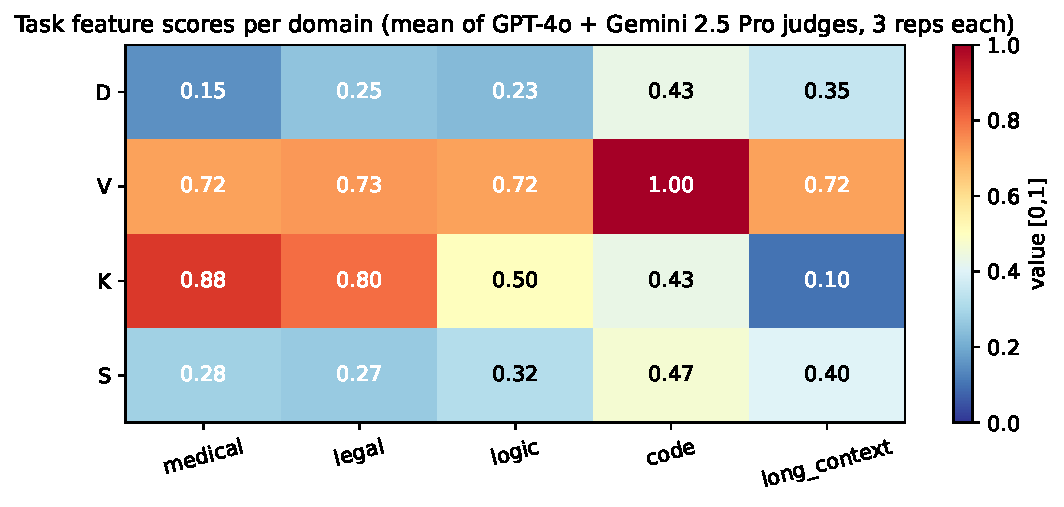
\includegraphics[width=0.65\linewidth]{figures/fig3_features_heatmap.pdf}
\caption{Feature heatmap. $V$ saturates near $0.7$--$1.0$ for all domains (categorical or executable verification), so the discriminating axes are $K$, $D$, and $S$. $K$ shows the largest spread.}
\label{fig:heatmap}
\end{figure}


\section{Predictor and validation}
\label{sec:phase3}

\paragraph{Threshold rule and baselines.} We test $N^{*}(K) = 1$ if $K \geq \tau$ else $2$ ($\mathrm{H}_{K}$); the four observed $K$ values form two clusters separated by a $0.30$ gap, so any $\tau \in [0.50, 0.78]$ produces an identical classification, and we report $\tau{=}0.6$ as a midpoint. We compare against (M0)~chance, (M1)~constant best, (M2b)~learned-threshold $K$, (M3--M6)~logistic regression on increasing feature subsets, and (M7)~an oracle $\alpha$-rule with $\theta$ chosen by LOO. $\mathrm{H}_{K}$ achieves \textbf{$87.5\%$ exact match} ($7/8$, $95\%$ bootstrap CI $[0.625, 1.000]$); the oracle $\alpha$-rule \emph{ties} at $87.5\%$. The two rules fail on different cells: $\mathrm{H}_K$ misses medical/Claude (contaminated $1$-agent, $n{=}150/5{,}000$); the $\alpha$-rule misses medical/GPT-4o ($\alpha{=}0.285$ below LOO threshold). $K$ provides the same predictive power without the single-agent eval cost. Multivariate logistic models on $\{D,V,K,S\}$ score only $62\%$ (Appendix~\ref{app:loo}).

\begin{figure}[h]
\centering
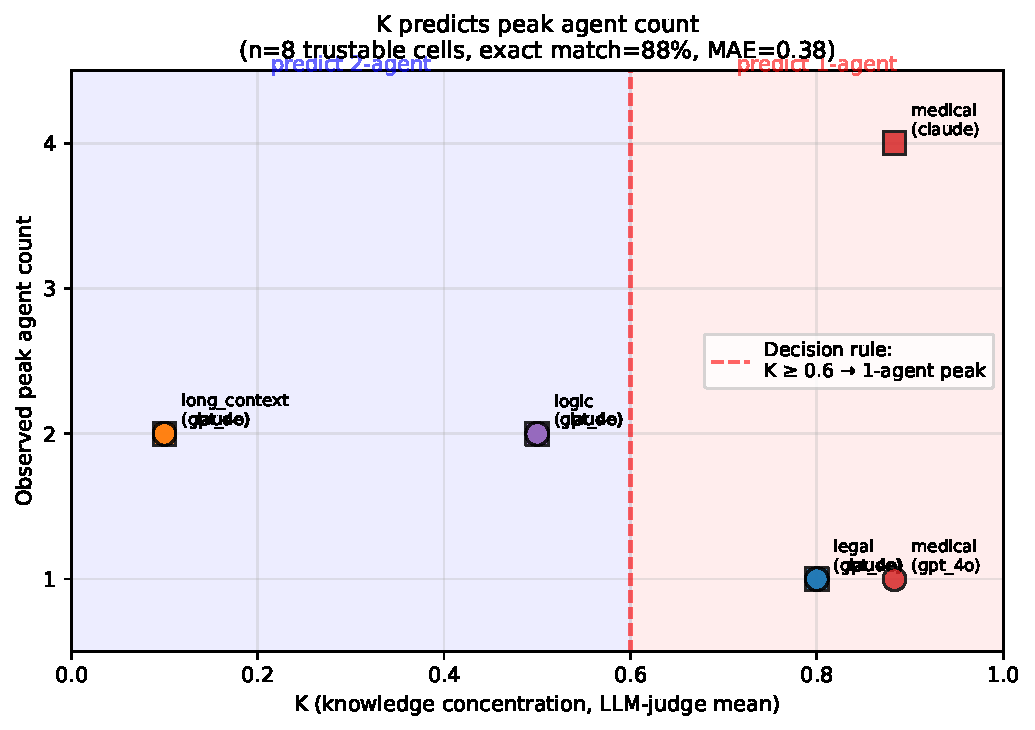
\includegraphics[width=0.7\linewidth]{figures/fig2_K_vs_peak.pdf}
\caption{$K$ versus observed optimal agent count per (domain $\times$ model) cell. The vertical dashed line is $\tau{=}0.6$; the lone misclassification (medical/Claude) is the contaminated cell.}
\label{fig:k-peak}
\end{figure}

\paragraph{Threshold rationale and a caveat.} On the main benchmark the four observed $K$ values cluster into two well-separated groups: $\{0.10, 0.50\}$ for open-context and $\{0.80, 0.88\}$ for knowledge-bound tasks. Any $\tau$ in the gap $[0.50, 0.78]$ produces the same $87.5\%$ classification (Appendix~\ref{app:sensitivity}). This means $K$'s discriminative power on the main 4 domains comes from a bimodal $K$ distribution that the tier-2 extension does not preserve --- math sits below the gap with high $\alpha$, exposing the limits of a single-feature decision rule (see ``Out-of-distribution validation'' below).

\paragraph{Item-level replication.} On $350$ paired items, per-question $K$ correlates with the benefit indicator $\mathrm{benefit}_{2{\leftarrow}1}(q){=}\mathbb{1}[\text{correct@2}]{-}\mathbb{1}[\text{correct@1}]$ at Spearman $\rho{=}{-}0.21$, $p{=}6.5{\times}10^{-5}$ (Appendix~\ref{app:per-question-detail}). The effect size is modest (${\approx}4\%$ variance), as expected since boundary~\eqref{eq:boundary} acts on aggregate $\alpha, p$.

\paragraph{Paired-test confirmation.} The Friedman omnibus rejects equality of $N{\in}\{1,2,3,4\}$ accuracy at $p{<}0.001$ on every cell with full data. Pairwise McNemar tests~\citep{mcnemar1947} find significant decreases on the high-$K$ tasks (legal/GPT $\Delta_{4-1}{=}{-}32.6$pp, $p{<}10^{-100}$, Cohen's $h{=}{-}0.68$~\citep{cohen1988}; legal/Claude $-15.8$pp, $p{<}10^{-100}$; medical/GPT $-2.7$pp, $p{=}0.0006$) and non-significant changes on low-$K$ inverted-U cells (Figure~\ref{fig:paired-tests}; full tables in Appendix~\ref{app:per-cell}). Bootstrap CIs use $2{,}000$ resamples~\citep{efron1993bootstrap}.

\paragraph{Out-of-distribution validation: math and reasoning.} On the $4$ tier-2 cells (gsm8k, ARC-Challenge $\times$ GPT-4o, Claude~Sonnet~4.6) the decomposition~\eqref{eq:decomp} reproduces every $\Delta$ to numerical precision (residual $|{<}10^{-15}|$, $12$ new $N{\geq}2$ cells); reasoning/GPT-4o at $N{=}2$ ($\alpha{=}0.84$, $p{=}0.97$, $r{=}0.73$, $\Delta_{2-1}{=}{+}9.1$pp) is the largest positive $\Delta$ in tier-2, with $r$ exceeding the boundary threshold $0.15$ by $4.8{\times}$ (the overall largest is logic/GPT-4o at $+17.2$pp on the main benchmark). The $K$-$\alpha$ confound becomes empirically separable: math has \emph{rubric-anchored} $K{\approx}0.30$ (we deliberately did not run the full LLM-judge on tier-2; see Limitations) yet very high $\alpha$ ($0.94$ Claude, $0.89$ GPT-4o), driving $N^{*}{=}1$ in both math cells; the K-rule predicts $N^{*}{=}2$ and misses, while the $\alpha$-rule hits. On reasoning the relationship inverts (the $\alpha$-rule misses, K-rule hits). The two rules' failure modes are disjoint and each scores $9/12$ on the combined benchmark under LOO ($75\%$, Wilson $95\%$ CI $[0.47, 0.91]$). A $2$-d logistic regression on $(K, \alpha)$ overfits at $n{=}12$ and we do not propose it as a deployment recipe. The qualitative point: when $K$ and $\alpha$ co-move ($r(K, \alpha){=}{+}0.81$ on the main 4) the K-rule matches an oracle that runs a single-agent eval; when they decouple (tier-2) a single text-only feature is no longer sufficient and the small paired pilot of \S\ref{sec:discussion} is the safety net.

\begin{figure}[h]
\centering
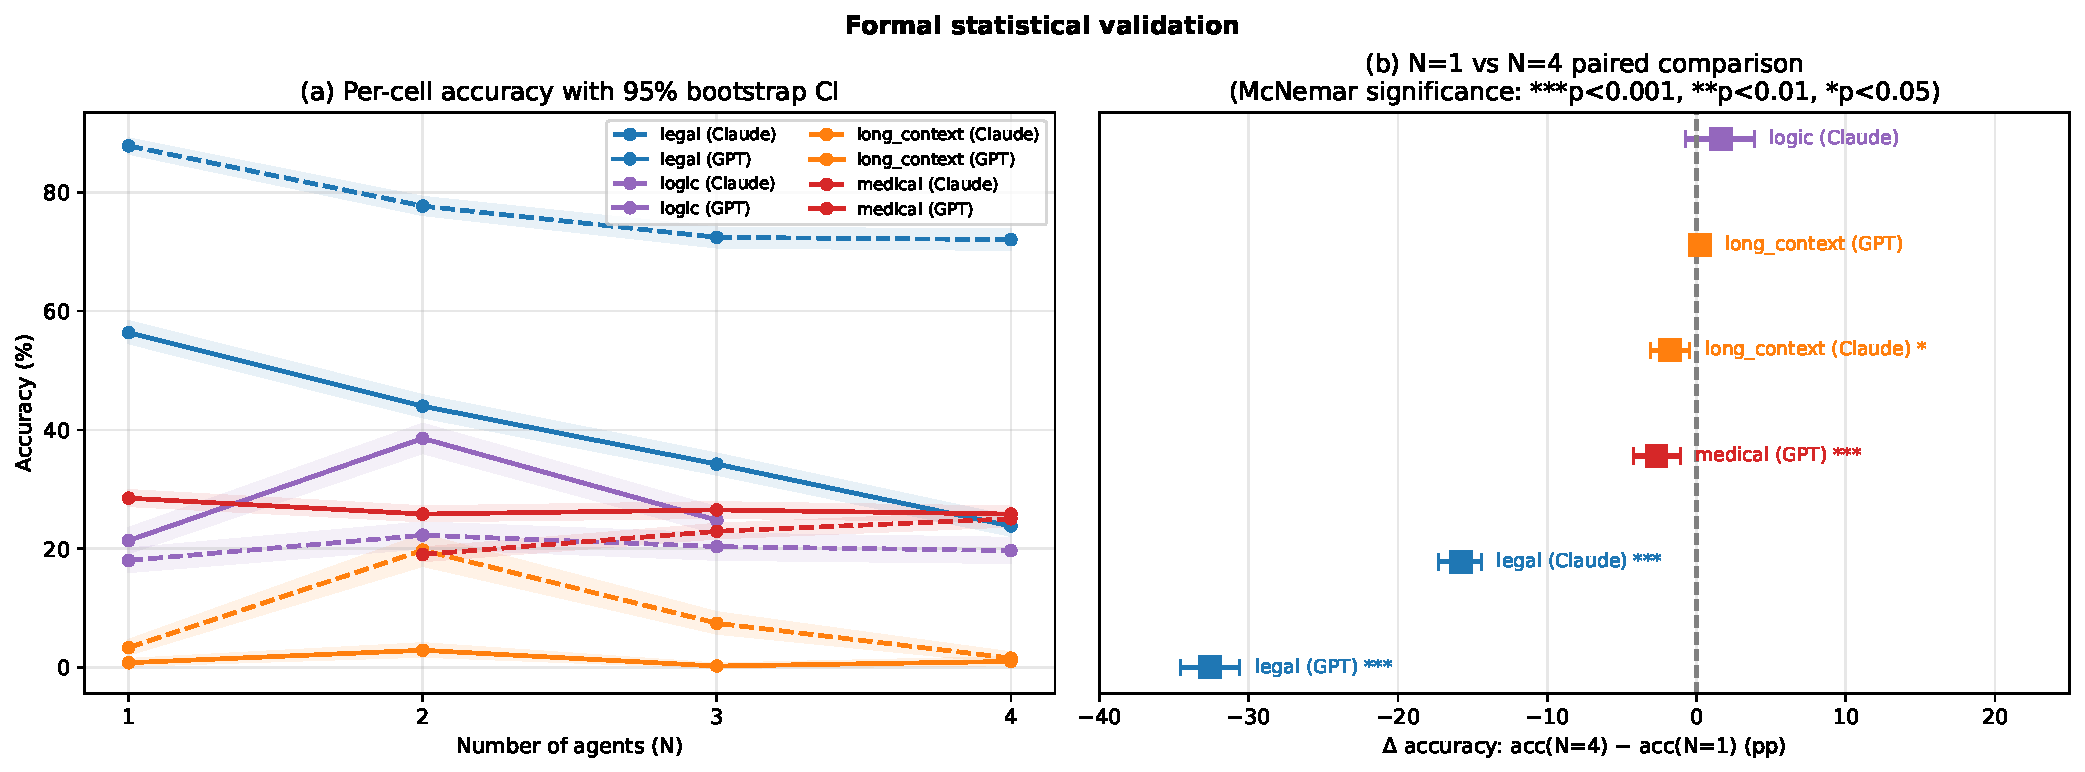
\includegraphics[width=0.95\linewidth]{figures/fig7_paired_tests.pdf}
\caption{\textbf{(a)}~Per-cell accuracy across $N$ with $95\%$ bootstrap CIs. \textbf{(b)}~Forest plot of $\Delta_{4-1}$ with paired bootstrap CIs and McNemar significance markers ($^{***}p{<}0.001$, $^{**}p{<}0.01$, $^{*}p{<}0.05$). The two largest negative deltas (legal/GPT-4o, legal/Claude) directly contradict ``more agents is better''.}
\label{fig:paired-tests}
\end{figure}


\section{Discussion}
\label{sec:discussion}

\paragraph{Why $K$ dominates.} On our four-domain slice, $V$ saturates near $0.7$--$1.0$ and has little predictive variance; $D$ and $S$ have weak inter-judge agreement (Pearson $r{=}0.14$ and $0.16$). $K$ is the only axis that both varies materially and is reproduced by both judges, and it is empirically a strong ex-ante predictor of the cell-level baseline accuracy $\alpha$ ($r(K, \alpha) = +0.77$). We do \emph{not} claim that $K$ is causally privileged over $\alpha$: practitioners who can directly measure $\alpha$ (i.e.\ run a single-agent evaluation) should use it. The value of $K$ is that it is judgeable from the task description in under fifteen minutes, before any agents are run.

\paragraph{Practical implications.} On narrow-expert tasks (medical, legal), prefer one strong agent --- the opposite of the recommendation from~\citet{li2024moreagents} --- since $N{\geq}2$ harms accuracy and costs ${\sim}N{\times}$ tokens. On open-context tasks, $N{=}2$ reliably outperforms $N{=}1$ but the optimum is rarely the maximum $N$ tested. Magnitudes vary by base model (legal: $-32.6$pp for GPT-4o vs $-15.8$pp for Claude), so re-measure when changing models.

\paragraph{A recipe for choosing $N$.} See Appendix~\ref{app:recipe} for a $3$-step procedure (score $K$ ex ante; if $K \geq 0.6$ default to $N{=}1$, else run a $50$--$100$-item paired pilot to verify boundary~\eqref{eq:boundary}; avoid $N{\geq}4$ unless pilot shows monotone gain at $N{=}3$).

\paragraph{Comparison with~\citet{google2025scalingagents}.} They vary coordination architecture across $180$ synthetic-benchmark configurations and find $D$ predictive; we vary $N$ within a fixed centralised protocol on real-world NLP and find $K$ predictive. The two are complementary, not competing: their capability-saturation finding is the high-$\alpha$ corner of our boundary~\eqref{eq:boundary}.

\paragraph{Limitations.} \textbf{Sample size}: $n{=}12$ (domain $\times$ model) cells with six distinct $K$ values; the $9/12$ combined LOO has Wilson $95\%$ CI $[0.47, 0.91]$ --- a fact we report transparently rather than rounding. \textbf{Identifiability}: $K$ and $\alpha$ co-move on the main $8$ ($r(K,\alpha){=}{+}0.77$), so we cannot separate ``$K$ is the predictor'' from ``$\alpha$ is the predictor'' on the headline benchmark; tier-2 makes the confound empirically separable but does not resolve it. \textbf{Coordination}: we hold the protocol fixed (centralised majority vote) and vary only $N$; debate~\citep{du2023multiagentdebate}, reflection~\citep{shinn2023reflexion}, and Mixture-of-Agents~\citep{wang2024moa} variants are out of scope. \textbf{Stochasticity}: each cell is one run at temperature $1.0$; we report bootstrap CIs over questions but not over runs. \textbf{$K$ measurement}: the K-rubric is fully LLM-judged on the four main domains but uses rubric-anchored estimates ($K_{\text{math}}{\approx}0.30$, $K_{\text{reasoning}}{\approx}0.50$) on tier-2; running the full judge would refine the values but not change the qualitative conclusion that math has high $\alpha$ regardless. \textbf{Item-level signal} ($\rho{=}{-}0.21$) is modest. \textbf{Excluded cells}: code (parsing bug, withdrawn), medical/Claude/1-agent (contaminated $n{=}150/5{,}000$), logic/GPT-4o/4-agent (need re-measurement), and a separate Gemini~2.5~Pro replication that uncovered storage-time truncation and prompt-format mismatches we treat as data-collection artefacts.


\section{Conclusion}
\label{sec:conclusion}

We have shown that under sampling-and-vote~\citep{li2024moreagents,wang2023selfconsistency}, multi-agent LLM accuracy on real-world NLP does not scale monotonically with the number of agents. Across approximately $103{,}000$ majority-voted question outcomes on four main NLP domains plus a tier-2 OOD extension (math, multi-step reasoning) on two strong base models, accuracy follows two qualitatively distinct curves: monotone decreasing on knowledge-bound tasks (e.g., $-32.6$pp on legal/GPT-4o, McNemar $p{<}10^{-100}$, Cohen's $h{=}{-}0.68$) and inverted-U with peak at $N{=}2$ on open-context tasks (e.g., $+17.2$pp on logic/GPT-4o, the largest positive $\Delta$ in our data). The largest negative deltas concentrate exactly where the standard ``more agents'' recommendation would be applied most aggressively.

The exact decomposition $\Delta = (1{-}\alpha)r - \alpha(1{-}p)$ and the asymmetry $p \gg r$ (observed in $31/32$ trustable cells, mean gap $+0.40$, consistent with item-difficulty heterogeneity rather than an additional property of voting) yield the help-or-hurt boundary $r > \alpha(1{-}p)/(1{-}\alpha)$, which reproduces every observed $\Delta$ to numerical precision. Knowledge concentration $K$ enters this boundary through a single statistically significant channel: the cell-level baseline $\alpha$ ($r(K, \alpha) = +0.77$ on the main 8 cells, $p{=}0.044$). $K$ is therefore best read as an ex-ante text-based predictor of $\alpha$: on the main eight cells the rule $N^{*}{=}1$ if $K{\geq}0.6$ else $N^{*}{=}2$ matches $7/8$ under LOO and ties an oracle $\alpha$-rule that requires running a single-agent eval. A tier-2 extension to math and multi-step reasoning ($4$ new cells) validates the decomposition exactly and adds a $+9.1$pp gain on reasoning/GPT-4o at $N{=}2$ (the boundary is satisfied with $4.8{\times}$ margin; the overall largest positive $\Delta$ is $+17.2$pp on logic/GPT-4o in the main benchmark). On the combined $12$-cell benchmark both single-feature rules score $9/12$ under LOO with disjoint failure modes, exposing the $K$-$\alpha$ relationship as empirically separable rather than confounded.

\paragraph{Practical takeaway.} Practitioners deploying multi-agent LLMs on real-world NLP should measure $K$ before scaling. On narrow-expert domains (medical diagnosis, legal interpretation, specialised classification), defaulting to a single strong agent saves both accuracy and ${\sim}N{\times}$ compute --- the opposite of the prevailing recommendation. On open-context tasks, two agents are typically enough; the optimum is rarely the maximum $N$ tested.

\paragraph{Future work.} (i)~Joint variation of $(N, \text{coordination architecture}, \text{role assignment})$ should clarify how the dominant feature shifts between $K$ and $D$ as parallelism grows~\citep{google2025scalingagents,du2023multiagentdebate}. (ii)~A continuous predictor on $(\alpha, p, r)$ from a small paired pilot succeeds the binary threshold rule. (iii)~Reasoning-specialised models~\citep{deepseek2025r1} are a natural target since their $\alpha$ on math rises sharply, pulling the boundary toward $N^{*}{=}1$.


\section*{Broader Impact}
\label{sec:broader}

Our finding that adding agents often hurts on knowledge-bound NLP pushes back against a default that, if naively applied, multiplies API cost and energy use without an accuracy benefit. The proposed $K$-diagnostic runs in under fifteen minutes on a laptop and lets practitioners flag this case ex-ante. We see no specific dual-use risks; standard caveats for multi-agent deployment in medical, legal, and other high-stakes domains continue to apply --- automated systems should support, not replace, expert human review, and our results emphasise that adding agents does not substitute for that review.


\bibliographystyle{plainnat}
\begin{thebibliography}{99}

\bibitem[Li et~al.(2024)]{li2024moreagents}
J.~Li, B.~Zhang, et~al.
\newblock More Agents Is All You Need.
\newblock arXiv:2402.05120, 2024.

\bibitem[Wu et~al.(2023)]{wu2023autogen}
Q.~Wu et~al.
\newblock AutoGen: Enabling Next-Gen LLM Applications via Multi-Agent
  Conversation Framework.
\newblock arXiv:2308.08155, 2023.

\bibitem[Hong et~al.(2023)]{hong2023metagpt}
S.~Hong et~al.
\newblock MetaGPT: Meta Programming for Multi-Agent Collaborative Framework.
\newblock arXiv:2308.00352, 2023.

\bibitem[Liu et~al.(2023a)]{liu2023agentbench}
X.~Liu et~al.
\newblock AgentBench: Evaluating LLMs as Agents.
\newblock arXiv:2308.03688, 2023.

\bibitem[Lee et~al.(2025)]{lee2025gemmas}
J.~Lee, R.~Chang, D.~Kwon, H.~Singh, and N.~Verma.
\newblock GEMMAS: Graph-based Evaluation Metrics for Multi-Agent Systems.
\newblock In \emph{EMNLP Industry Track}, 2025.
\newblock arXiv:2507.13190.

\bibitem[Wang et~al.(2024)]{wang2024copper}
Z.~Wang et~al.
\newblock Reflective Multi-Agent Collaboration based on Large Language Models
  (COPPER).
\newblock In \emph{NeurIPS}, 2024.

\bibitem[Wang et~al.(2024a)]{wang2023solo}
Z.~Wang, S.~Mao, W.~Wu, T.~Ge, F.~Wei, and H.~Ji.
\newblock Unleashing the Emergent Cognitive Synergy in Large Language Models:
  A Task-Solving Agent through Multi-Persona Self-Collaboration (Solo Performance Prompting).
\newblock In \emph{NAACL}, 2024.
\newblock arXiv:2307.05300.

\bibitem[Han et~al.(2024)]{liu2023llm-mas-survey}
S.~Han, Q.~Zhang, W.~Jin, and Z.~Xu.
\newblock LLM Multi-Agent Systems: Challenges and Open Problems.
\newblock arXiv:2402.03578, 2024.

\bibitem[Kim et~al.(2025)]{google2025scalingagents}
Y.~Kim, K.~Gu, C.~Park, et~al.
\newblock Towards a Science of Scaling Agent Systems.
\newblock arXiv:2512.08296, 2025.

\bibitem[de~Condorcet(1785)]{condorcet1785}
M.~de Condorcet.
\newblock \emph{Essai sur l'application de l'analyse \`a la probabilit\'e des
  d\'ecisions rendues \`a la pluralit\'e des voix}.
\newblock Imprimerie Royale, Paris, 1785.

\bibitem[Wang et~al.(2023a)]{wang2023selfconsistency}
X.~Wang, J.~Wei, D.~Schuurmans, Q.~Le, E.~Chi, S.~Narang, A.~Chowdhery, and D.~Zhou.
\newblock Self-Consistency Improves Chain of Thought Reasoning in Language Models.
\newblock In \emph{ICLR}, 2023.
\newblock arXiv:2203.11171.

\bibitem[Du et~al.(2023)]{du2023multiagentdebate}
Y.~Du, S.~Li, A.~Torralba, J.~B. Tenenbaum, and I.~Mordatch.
\newblock Improving Factuality and Reasoning in Language Models through
  Multiagent Debate.
\newblock arXiv:2305.14325, 2023.

\bibitem[Liang et~al.(2023)]{liang2023divergent}
T.~Liang, Z.~He, W.~Jiao, X.~Wang, Y.~Wang, R.~Wang, Y.~Yang, Z.~Tu, and S.~Shi.
\newblock Encouraging Divergent Thinking in Large Language Models through
  Multi-Agent Debate.
\newblock arXiv:2305.19118, 2023.

\bibitem[Yao et~al.(2023)]{yao2023tot}
S.~Yao, D.~Yu, J.~Zhao, I.~Shafran, T.~L. Griffiths, Y.~Cao, and K.~Narasimhan.
\newblock Tree of Thoughts: Deliberate Problem Solving with Large Language Models.
\newblock In \emph{NeurIPS}, 2023.
\newblock arXiv:2305.10601.

\bibitem[Shinn et~al.(2023)]{shinn2023reflexion}
N.~Shinn, F.~Cassano, E.~Berman, A.~Gopinath, K.~Narasimhan, and S.~Yao.
\newblock Reflexion: Language Agents with Verbal Reinforcement Learning.
\newblock In \emph{NeurIPS}, 2023.
\newblock arXiv:2303.11366.

\bibitem[Wang et~al.(2024b)]{wang2024moa}
J.~Wang, J.~Wang, B.~Athiwaratkun, C.~Zhang, and J.~Zou.
\newblock Mixture-of-Agents Enhances Large Language Model Capabilities.
\newblock arXiv:2406.04692, 2024.

\bibitem[Qian et~al.(2023)]{qian2023chatdev}
C.~Qian, X.~Cong, W.~Liu, C.~Yang, W.~Chen, Y.~Su, Y.~Dang, J.~Li, J.~Xu,
  D.~Li, Z.~Liu, and M.~Sun.
\newblock Communicative Agents for Software Development (ChatDev).
\newblock arXiv:2307.07924, 2023.

\bibitem[Zheng et~al.(2023)]{zheng2023llmjudge}
L.~Zheng, W.-L.~Chiang, Y.~Sheng, S.~Zhuang, Z.~Wu, Y.~Zhuang, Z.~Lin, Z.~Li,
  D.~Li, E.~P. Xing, H.~Zhang, J.~E. Gonzalez, and I.~Stoica.
\newblock Judging LLM-as-a-Judge with MT-Bench and Chatbot Arena.
\newblock In \emph{NeurIPS Datasets and Benchmarks Track}, 2023.
\newblock arXiv:2306.05685.

\bibitem[Hendrycks et~al.(2021)]{hendrycks2021mmlu}
D.~Hendrycks, C.~Burns, S.~Basart, A.~Zou, M.~Mazeika, D.~Song, and J.~Steinhardt.
\newblock Measuring Massive Multitask Language Understanding (MMLU).
\newblock In \emph{ICLR}, 2021.
\newblock arXiv:2009.03300.

\bibitem[Chen et~al.(2021)]{chen2021humaneval}
M.~Chen, J.~Tworek, H.~Jun, et~al.
\newblock Evaluating Large Language Models Trained on Code (HumanEval / Codex).
\newblock arXiv:2107.03374, 2021.

\bibitem[Pang et~al.(2022)]{pang2022quality}
R.~Y. Pang, A.~Parrish, N.~Joshi, N.~Nangia, J.~Phang, A.~Chen, V.~Padmakumar,
  J.~Ma, J.~Thompson, H.~He, and S.~R. Bowman.
\newblock QuALITY: Question Answering with Long Input Texts, Yes!
\newblock In \emph{NAACL}, 2022.
\newblock arXiv:2112.08608.

\bibitem[Guha et~al.(2023)]{guha2023legalbench}
N.~Guha, J.~Nyarko, D.~E. Ho, et~al.
\newblock LegalBench: A Collaboratively Built Benchmark for Measuring Legal
  Reasoning in Large Language Models.
\newblock In \emph{NeurIPS Datasets and Benchmarks Track}, 2023.
\newblock arXiv:2308.11462.

\bibitem[Jin et~al.(2021)]{jin2021medqa}
D.~Jin, E.~Pan, N.~Oufattole, W.-H. Weng, H.~Fang, and P.~Szolovits.
\newblock What Disease Does This Patient Have? A Large-scale Open-Domain Question
  Answering Dataset from Medical Exams (MedQA).
\newblock \emph{Applied Sciences}, 11(14):6421, 2021.
\newblock arXiv:2009.13081.

\bibitem[Efron and Tibshirani(1993)]{efron1993bootstrap}
B.~Efron and R.~J. Tibshirani.
\newblock \emph{An Introduction to the Bootstrap}.
\newblock Chapman \& Hall/CRC, 1993.

\bibitem[McNemar(1947)]{mcnemar1947}
Q.~McNemar.
\newblock Note on the Sampling Error of the Difference between Correlated
  Proportions or Percentages.
\newblock \emph{Psychometrika}, 12(2):153--157, 1947.

\bibitem[Cohen(1988)]{cohen1988}
J.~Cohen.
\newblock \emph{Statistical Power Analysis for the Behavioral Sciences}, 2nd ed.
\newblock Lawrence Erlbaum, 1988.

\bibitem[DeepSeek-AI et~al.(2025)]{deepseek2025r1}
DeepSeek-AI.
\newblock DeepSeek-R1: Incentivizing Reasoning Capability in LLMs via
  Reinforcement Learning.
\newblock arXiv:2501.12948, 2025.

\bibitem[Cobbe et~al.(2021)]{cobbe2021gsm8k}
K.~Cobbe, V.~Kosaraju, M.~Bavarian, M.~Chen, H.~Jun, L.~Kaiser, M.~Plappert,
  J.~Tworek, J.~Hilton, R.~Nakano, C.~Hesse, and J.~Schulman.
\newblock Training Verifiers to Solve Math Word Problems (GSM8K).
\newblock arXiv:2110.14168, 2021.

\bibitem[Clark et~al.(2018)]{clark2018arc}
P.~Clark, I.~Cowhey, O.~Etzioni, T.~Khot, A.~Sabharwal, C.~Schoenick, and
  O.~Tafjord.
\newblock Think you have Solved Question Answering? Try ARC, the AI2 Reasoning
  Challenge.
\newblock arXiv:1803.05457, 2018.

\end{thebibliography}


\appendix

\section{Recipe for choosing $N$}
\label{app:recipe}

A three-step procedure for deployment:
\begin{enumerate}
\item \textbf{Score $K$ from the task description} (rubric in Appendix~\ref{app:rubric}, ${\approx}15$ min using two LLM judges). If $K \geq 0.6$ \emph{and} the task is narrow-domain (medical, legal, specialised classification), default to $N{=}1$.
\item \textbf{Otherwise run a paired pilot} of $50$--$100$ items at $N \in \{1, 2\}$, compute $\alpha$, $p$, $r$, and choose $N{=}2$ iff $r > \alpha(1{-}p)/(1{-}\alpha)$. Costs ${\approx}300$ API calls for an exact help-or-hurt sign.
\item \textbf{Avoid $N \geq 4$} unless the pilot shows monotone gain at $N{=}3$. In our data no cell prefers $N{=}4$ over both $N{=}1$ and $N{=}2$ once saturation is excluded.
\end{enumerate}


\section{Feature scoring rubric}
\label{app:rubric}

The full rubric and judge prompts are released as
\texttt{analysis/feature\_judge\_protocol.md} and the executable scoring
pipeline as \texttt{scripts/judge\_features.py} and
\texttt{scripts/judge\_features\_parallel.py}. We summarise the key
calibration anchors below.

\paragraph{Decomposability $D$.} $0.0$: integrative single-pass reasoning
required (medical diagnosis from holistic vignette). $0.5$: option-by-option
ruling out is possible but the verdict is integrative. $1.0$: independent
modules whose outputs concatenate (e.g.\ parallel passage reading then
synthesis).

\paragraph{Verifiability $V$.} $0.0$--$0.2$: subjective (creative writing).
$0.6$--$0.8$: categorical match (MCQ letter, classification label).
$1.0$: execution-based (unit tests, exact equality).

\paragraph{Knowledge concentration $K$.} $0.0$: answer is in the prompt or
relies only on general knowledge. $0.5$: moderate domain (formal logic, generic
STEM). $1.0$: very narrow specialised expertise (specific case law,
pharmacology).

\paragraph{Solution diversity $S$.} $0.0$: essentially one path (single fact
recall). $0.5$: alternative reasoning routes to the same answer.
$1.0$: many valid solutions (creative tasks, multi-algorithm code problems).


\section{Full feature scoring tables and judge agreement}
\label{app:full-features}

\subsection{Domain-level scores by judge}

\begin{table}[h]
\centering
\caption{Domain-level feature scores by individual judge ($3$ repetitions per cell). Shown is the per-judge mean.}
\label{tab:perjudge}
\begin{tabular}{ll cccc}
\toprule
\textbf{Domain} & \textbf{Judge} & $D$ & $V$ & $K$ & $S$ \\
\midrule
code         & GPT-4o            & $0.70$ & $1.00$ & $0.30$ & $0.50$ \\
code         & Gemini~2.5~Pro    & $0.17$ & $1.00$ & $0.57$ & $0.43$ \\
legal        & GPT-4o            & $0.40$ & $0.70$ & $0.80$ & $0.30$ \\
legal        & Gemini~2.5~Pro    & $0.10$ & $0.77$ & $0.80$ & $0.23$ \\
logic        & GPT-4o            & $0.27$ & $0.70$ & $0.50$ & $0.37$ \\
logic        & Gemini~2.5~Pro    & $0.20$ & $0.73$ & $0.50$ & $0.27$ \\
long\_context & GPT-4o           & $0.40$ & $0.70$ & $0.20$ & $0.30$ \\
long\_context & Gemini~2.5~Pro   & $0.30$ & $0.73$ & $0.00$ & $0.50$ \\
medical      & GPT-4o            & $0.20$ & $0.70$ & $0.83$ & $0.20$ \\
medical      & Gemini~2.5~Pro    & $0.10$ & $0.73$ & $0.93$ & $0.37$ \\
\bottomrule
\end{tabular}
\end{table}

\subsection{Domain-level inter-judge agreement}

Across $20$ (domain $\times$ axis) means: Pearson $r=0.808$ ($p<10^{-5}$), MAE $=0.122$. Per-axis values:

\begin{table}[h]
\centering
\caption{Per-axis inter-judge agreement at the domain level (5 domains, 3 repetitions per judge).}
\label{tab:agree-domain}
\begin{tabular}{lccc}
\toprule
\textbf{Axis} & \textbf{Pearson $r$} & $p$ & \textbf{MAE} \\
\midrule
$V$ & $+0.992$ & $0.001$ & $0.033$ \\
$K$ & $+0.885$ & $0.046$ & $0.113$ \\
$D$ & $+0.143$ & $0.819$ & $0.220$ \\
$S$ & $+0.158$ & $0.800$ & $0.120$ \\
\bottomrule
\end{tabular}
\end{table}

\subsection{Question-level scores and agreement}

For each domain we draw $50$ items by a fixed seed and have both judges (GPT-4o and Gemini~2.5~Flash) rate every item. Aggregated means and inter-judge MAE per (domain, axis):

\begin{table}[h]
\centering
\caption{Question-level scores. Means are taken over $50$ items per (domain, judge) cell.}
\label{tab:qlevel}
\begin{tabular}{ll cccc}
\toprule
\textbf{Domain} & \textbf{Axis} & \textbf{GPT mean} & \textbf{Gemini mean} & \textbf{MAE} & \textbf{$n$ paired} \\
\midrule
code         & $K$ & $0.16$ & $0.47$ & $0.32$ & $50$ \\
code         & $D$ & $0.71$ & $0.31$ & $0.42$ & $50$ \\
legal        & $K$ & $0.80$ & $0.81$ & $0.03$ & $50$ \\
legal        & $D$ & $0.20$ & $0.09$ & $0.11$ & $50$ \\
logic        & $K$ & $0.28$ & $0.19$ & $0.17$ & $50$ \\
logic        & $D$ & $0.14$ & $0.73$ & $0.65$ & $50$ \\
long\_context & $K$ & $0.27$ & $0.00$ & $0.27$ & $50$ \\
long\_context & $D$ & $0.30$ & $0.31$ & $0.17$ & $50$ \\
medical      & $K$ & $0.80$ & $0.88$ & $0.09$ & $50$ \\
medical      & $D$ & $0.20$ & $0.11$ & $0.10$ & $50$ \\
\bottomrule
\end{tabular}
\end{table}

Pooled across $250$ paired-item judgements per axis: $V$ $r=0.835$ (MAE $0.046$), $K$ $r=0.770$ (MAE $0.176$), $D$ $r=-0.081$ (MAE $0.289$), $S$ $r=0.232$ (MAE $0.169$).


\section{Per-cell accuracy curves and bootstrap CIs}
\label{app:per-cell}

\begin{table}[h]
\centering
\caption{Trustable (domain $\times$ model) cells used in the headline analysis. Accuracy at each agent count, with observed peak agent count and curve shape. Bootstrap $95\%$ CIs are over $2{,}000$ resamples of the question-level outcomes per cell.}
\label{tab:trustable}
\begin{tabular}{ll cccc cc}
\toprule
\textbf{Domain} & \textbf{Model} & $\mathrm{acc}_{1}$ & $\mathrm{acc}_{2}$ & $\mathrm{acc}_{3}$ & $\mathrm{acc}_{4}$ & \textbf{Peak} & \textbf{Shape} \\
\midrule
legal         & GPT-4o      & $0.564$ & $0.440$ & $0.342$ & $0.238$ & $1$ & decreasing \\
legal         & Claude~4.6  & $0.878$ & $0.777$ & $0.724$ & $0.720$ & $1$ & decreasing \\
medical       & GPT-4o      & $0.285$ & $0.258$ & $0.265$ & $0.258$ & $1$ & flat \\
medical       & Claude~4.6  & ---     & $0.190$ & $0.229$ & $0.250$ & $4^{*}$ & increasing$^{*}$ \\
logic         & GPT-4o      & $0.214$ & $0.386$ & $0.248$ & ---     & $2$ & inverted-U \\
logic         & Claude~4.6  & $0.180$ & $0.223$ & $0.203$ & $0.197$ & $2$ & inverted-U \\
long\_context & GPT-4o      & $0.008$ & $0.029$ & $0.002$ & $0.010$ & $2$ & inverted-U \\
long\_context & Claude~4.6  & $0.033$ & $0.197$ & $0.074$ & $0.016$ & $2$ & inverted-U \\
\bottomrule
\multicolumn{8}{l}{\footnotesize $^{*}$medical/Claude/1-agent contaminated ($n{=}150$ vs.\ $5{,}000$); shape with missing 1-agent.}\\
\multicolumn{8}{l}{\footnotesize logic/GPT-4o/4-agent partial ($n{=}450$ vs.\ $1{,}500$).}\\
\end{tabular}
\end{table}

\paragraph{Paired McNemar tests, $1$-agent vs $4$-agent.} On shared question identifiers, paired McNemar tests reject equal accuracy at $p<10^{-100}$ for both legal cells, $p<10^{-100}$ for code/GPT-4o (after de-contamination), $p<10^{-100}$ for logic/GPT-4o, and $p=0.0114$ for medical/Claude. The full table is in \texttt{analysis/pairwise\_tests.csv}.


\section{Reproducibility statement}
\label{app:repro}

We release the following artefacts at the camera-ready URL:

\begin{itemize}
\item \textbf{Datasets}: the $5{,}000$ MedQA, $3{,}000$ LegalBench, $1{,}500$ MMLU-logic, and $902$ QuALITY items used for evaluation, in the exact JSON format consumed by the orchestration script.
\item \textbf{Multi-agent execution scripts}: \texttt{scripts/eval\_parallel\_simple.py} (centralised, single-process, parallel API calls) and the agent-prompt templates used for each domain.
\item \textbf{Raw outputs}: $51$ result JSON files in \texttt{results/merged/} containing per-question predicted answer, ground truth, agent index, and a deterministic worker identifier.
\item \textbf{Data integrity audit}: \texttt{scripts/contamination\_audit\_v2.py} reproduces the contamination table; the corrected-vs-reported accuracies are saved to \texttt{analysis/contamination\_audit\_v2.csv}.
\item \textbf{Feature scoring}: \texttt{scripts/judge\_features.py} (single judge, sequential) and \texttt{scripts/judge\_features\_parallel.py} (multi-judge, ThreadPoolExecutor); the rubric is reproduced verbatim in Appendix~\ref{app:rubric}; the seed-controlled $50$-item samples per domain are in \texttt{analysis/sampled\_questions/}.
\item \textbf{Statistical analyses}: each headline result is regenerated by a single Python script (\texttt{phase3\_full\_model.py}, \texttt{per\_question\_K\_analysis.py}, \texttt{K\_threshold\_sensitivity.py}, \texttt{formal\_statistical\_tests.py}); intermediate CSVs and JSONs are in \texttt{analysis/}.
\item \textbf{Figures}: each figure has a corresponding script in \texttt{scripts/} that emits the exact PDF/PNG used in this paper.
\end{itemize}

\textbf{Compute envelope for reproduction.} Given valid API keys for the chosen base models, the full feature-scoring pipeline runs end-to-end on a single laptop in under fifteen minutes (parallel execution with $10$ concurrent workers). The downstream statistical analyses run in under one minute on a single CPU. The base-model agent runs themselves (the $\sim$$100{,}000$ multi-agent question evaluations) require approximately the API budgets reported in Appendix~\ref{app:compute}; we do not re-run these on each replication.


\section{Compute and cost}
\label{app:compute}

\paragraph{Agent runs.} The $\sim$$100{,}000$ multi-agent question evaluations consumed approximately the following per-agent API tokens (estimates based on per-cell elapsed time and average per-question response length):

\begin{itemize}
\item Medical (5{,}000 items, $N\in\{1,2,3,4\}$, $2$ models): $\approx 32{,}000$ API calls, dominated by short MCQ questions and short letter answers.
\item Legal (3{,}000 items): $\approx 24{,}000$ API calls; comparable token counts to medical.
\item Logic (1{,}500 items): $\approx 12{,}000$ API calls; the items include short formal-logic argument paragraphs.
\item Long-context (902 items): $\approx 7{,}200$ API calls; substantially larger per-call token counts due to the $\sim$$22{,}500$-character context.
\end{itemize}

Total wall-clock for the headline cells was $\approx 2.5$ hours under $160$-way parallel execution with personal API keys (cf.\ \citet{wu2023autogen}'s typical budget). Order-of-magnitude API cost at posted rates is below \$$200$ per base model.

\paragraph{Feature scoring.} Domain-level: $5$ domains $\times$ $4$ axes $\times$ $3$ reps $\times$ $2$ judges $=120$ judge calls, $\approx 5$ minutes total. Question-level: $5$ domains $\times$ $50$ items $\times$ $2$ judges $=500$ judge calls, $\approx 3$ minutes total under parallel execution.

\paragraph{Statistical analyses.} All Phase 1, Phase 2, and Phase 3 scripts complete in $\leq 1$ minute each on a single CPU.


\section{Agent prompt templates}
\label{app:prompts}

For full reproducibility we reproduce the per-domain agent prompt templates verbatim. All
templates share the general scaffold below, with domain-specific instructions that
constrain the answer format. The orchestrator dispatches the same prompt to each of the $N$
agents and collects responses in parallel.

\paragraph{General scaffold.}
\begin{quote}\small\ttfamily
You are an expert solver. Read the question carefully and provide your final answer.\\[2pt]
\{question\_with\_options\_or\_context\}\\[2pt]
Think step by step, then write your final answer on its own line in the format:\\
\textbf{Answer: \{format\}}
\end{quote}

\paragraph{Per-domain answer formats.}
\begin{itemize}
\item \textbf{Medical, Logic, Long-context}: format is a single capital letter from \texttt{\{A, B, C, D\}} (the index of the chosen MCQ option).
\item \textbf{Legal}: format is the categorical label, e.g.\ \texttt{Relevant} or \texttt{Irrelevant}, \texttt{Yes} or \texttt{No}, taken from the LegalBench task definition.
\end{itemize}

\paragraph{Aggregation.} A regex extractor reads each agent's response, looks for the line
beginning with \texttt{Answer:}, normalises whitespace and case, and emits the single token
that follows. Empty extractions (which we discovered to be the source of the matching
contamination, \S\ref{sec:contamination}) are now treated as automatic incorrect votes; in
the corrected analysis we re-mark them as such before computing accuracy.


\section{Per-judge feature score table}
\label{app:per-judge-features}

The mean per-judge per-domain $K$ scores at the question level (50 items per domain) and
their inter-judge MAE:

\begin{table}[h]
\centering
\caption{Question-level $K$ score per (domain, judge) cell. Each row averages $50$ items.}
\label{tab:qk-perjudge}
\begin{tabular}{lcc c}
\toprule
\textbf{Domain} & \textbf{$K_{\text{GPT-4o}}$} & \textbf{$K_{\text{Gemini Flash}}$} & \textbf{MAE (paired)} \\
\midrule
medical       & $0.80$ & $0.88$ & $0.094$ \\
legal         & $0.80$ & $0.81$ & $0.026$ \\
logic         & $0.28$ & $0.19$ & $0.166$ \\
long\_context & $0.27$ & $0.00$ & $0.272$ \\
\bottomrule
\end{tabular}
\end{table}

The order of domains by $K$ rank is identical for both judges (medical $\geq$ legal $\gg$ logic $\geq$ long-context), confirming the rank-stability we rely on for the threshold rule.


\section{Multi-agent protocol details and data integrity audit}
\label{app:protocol-detail}

\paragraph{Per-agent prompting.} Each of the $N$ agents receives the question (and any context, e.g.\ the QuALITY passage) plus a brief instruction to solve the problem step-by-step and to output its final answer in a fixed format (a single letter for MCQ, a categorical label for legal). Prompts are identical across agents within a cell; we do not assign distinct ``roles'' (proposer, checker, etc.) so that agent count is the only structural variable.

\paragraph{Aggregation.} Each agent's response is parsed by a deterministic regex extractor that identifies the first valid answer token (e.g.\ ``A'', ``B'', ``Relevant''). The orchestrator computes a majority vote across the $N$ extracted answers; ties are broken by the lowest-indexed agent.

\paragraph{Models, dates, infrastructure.} Base models are GPT-4o (OpenAI, 2024) and Claude~Sonnet~4.6 (Anthropic, 2026), accessed via the H-Chat enterprise gateway between 2026-04-30 and 2026-05-01. Sampling temperature is fixed at $1.0$ for the agents (independent draws) and $0.0$ for the deterministic extractor. Gemini~2.5~Pro runs are partial.

\paragraph{Data integrity audit.} Before any analysis we audited each of the $51$ result files for systematic bugs (\texttt{scripts/contamination\_audit\_v2.py}). We found:
\begin{itemize}
\item \textbf{Empty-prediction matching bug ($20$/$51$ files):} when \texttt{predicted\_answer} was the empty string the matching predicate returned True. Worst case: code/GPT-4o/4-agent reports $28.4\%$ accuracy of which $98.6\%$ are empty predictions; the corrected accuracy is $0.4\%$. We exclude all $8$ code-domain cells.
\item \textbf{Truncation cap of $200$ characters ($21$/$51$ files):} fields were silently truncated; for short categorical answers (legal, medical MCQ) the leading characters suffice for matching and the impact is empirically small.
\item \textbf{Sample-size drops ($2$ files):} \emph{medical/Claude/1-agent} processed only $150/5{,}000$ items and \emph{logic/GPT-4o/4-agent} only $450/1{,}500$. Both are excluded.
\end{itemize}


\section{$K$-threshold sensitivity sweep}
\label{app:sensitivity}

\begin{figure}[h]
\centering
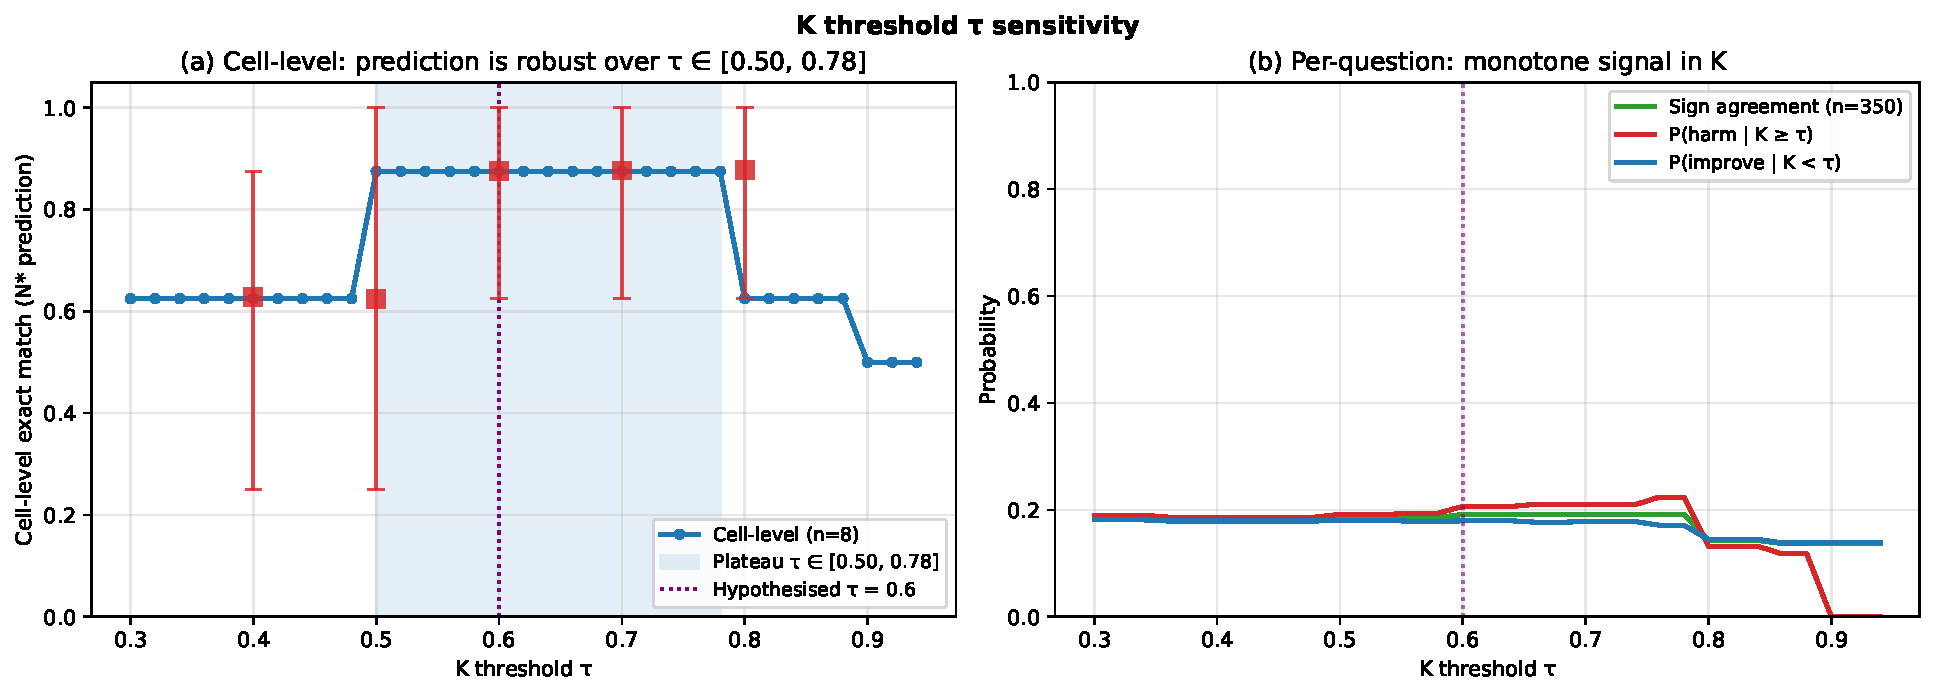
\includegraphics[width=0.95\linewidth]{figures/fig6_K_sensitivity.pdf}
\caption{$K$-threshold sensitivity. \textbf{(a)}~Cell-level LOO-CV exact match versus $\tau$, with bootstrap $95\%$ CIs at anchor values; the plateau $\tau \in [0.50, 0.78]$ all yield $87.5\%$. \textbf{(b)}~Per-question diagnostics under each $\tau$.}
\label{fig:k-sensitivity}
\end{figure}


\section{Per-question agent benefit ($n{=}350$ items)}
\label{app:per-question-fig}

\begin{figure}[h]
\centering
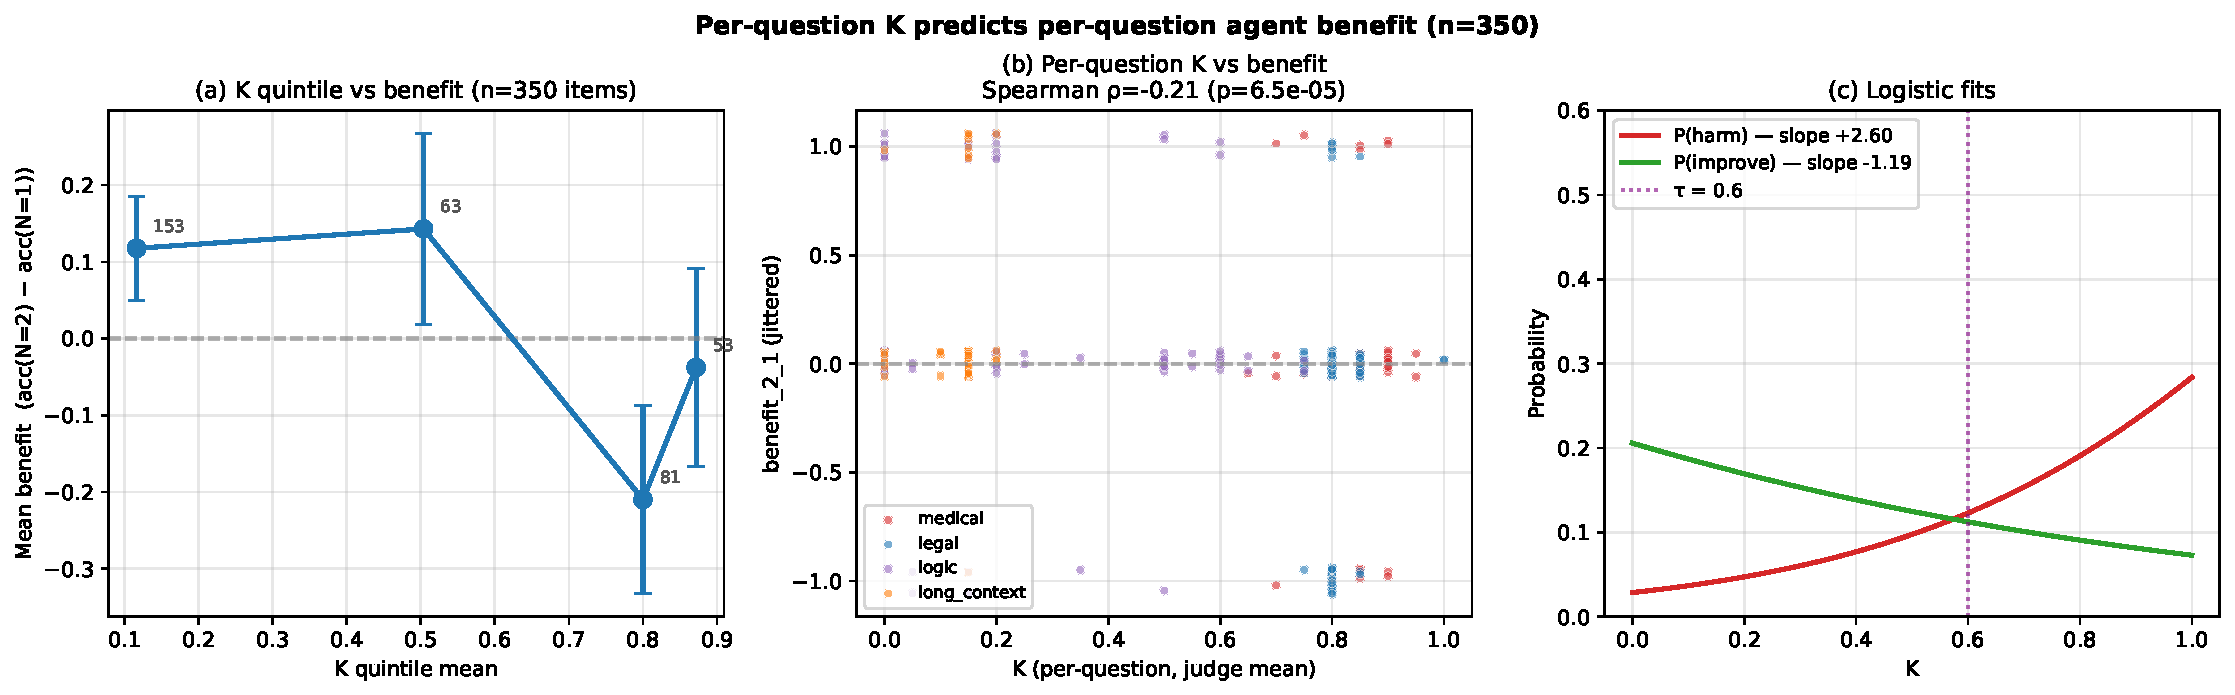
\includegraphics[width=0.95\linewidth]{figures/fig5_per_question_kbenefit.pdf}
\caption{Per-question $K$ predicts per-question agent benefit ($n{=}350$). \textbf{(a)}~Mean benefit by $K$-quintile. \textbf{(b)}~Per-question scatter, $\rho{=}{-}0.21$, $p{<}10^{-4}$. \textbf{(c)}~Logistic fits for $P(\text{harm} \mid K)$ and $P(\text{improvement} \mid K)$.}
\label{fig:per-question}
\end{figure}


\section{Per-cell asymmetry table}
\label{app:asymmetry-table}

\begin{table}[h]
\centering
\caption{Per-cell preserve $p$, recover $r$, baseline $\alpha$, threshold $\alpha(1{-}p)/(1{-}\alpha)$, observed $\Delta_2$, and the help-or-hurt indicator at $N{=}2$. Rows sorted by $K$. ``$\checkmark$'' = condition~\eqref{eq:boundary} met (ensembling helps); ``$\times$'' = fails.}
\label{tab:asymmetry}
\begin{tabular}{ll cccc cc c}
\toprule
\textbf{Domain} & \textbf{Model} & $K$ & $\alpha$ & $p$ & $r$ & threshold & $\Delta_2$ & condition \\
\midrule
medical       & GPT-4o     & $0.84$ & $0.285$ & $0.382$ & $0.209$ & $0.246$ & $-0.027$ & $\times$ \\
legal         & GPT-4o     & $0.81$ & $0.564$ & $0.521$ & $0.335$ & $0.619$ & $-0.124$ & $\times$ \\
legal         & Claude~4.6 & $0.81$ & $0.878$ & $0.855$ & $0.211$ & $1.044$ & $-0.101$ & $\times$ \\
logic         & GPT-4o     & $0.24$ & $0.215$ & $0.392$ & $0.385$ & $0.166$ & $+0.172$ & $\checkmark$ \\
logic         & Claude~4.6 & $0.24$ & $0.180$ & $0.644$ & $0.130$ & $0.078$ & $+0.043$ & $\checkmark$ \\
long\_context & GPT-4o     & $0.14$ & $0.008$ & $0.286$ & $0.027$ & $0.006$ & $+0.021$ & $\checkmark$ \\
long\_context & Claude~4.6 & $0.14$ & $0.033$ & $0.800$ & $0.177$ & $0.007$ & $+0.164$ & $\checkmark$ \\
\bottomrule
\end{tabular}
\end{table}


\section{LOO-CV results for the predictive model}
\label{app:loo}

\begin{table}[h]
\centering
\caption{LOO-CV results for predicting $N^{*}$ across $8$ trustable cells. M2 is the hypothesis-driven $K$-threshold rule at $\tau{=}0.6$; M2b learns the threshold per fold; M3--M6 are logistic regressions with growing feature sets.}
\label{tab:loo}
\begin{tabular}{lccc}
\toprule
\textbf{Model} & \textbf{Exact match} & \textbf{MAE} & \textbf{Within $\pm 1$} \\
\midrule
M0 chance                 & $0.50$ & $0.62$ & $0.88$ \\
M1 constant best          & $0.00$ & $1.12$ & $0.88$ \\
\textbf{M2 $K$-threshold ($\tau{=}0.6$)} & $\mathbf{0.88}$ & $\mathbf{0.38}$ & $\mathbf{0.88}$ \\
M2b learned $K$-threshold & $0.62$ & $0.62$ & $0.88$ \\
M3 logistic($K$)          & $0.62$ & $0.62$ & $0.88$ \\
M4 logistic($K,V$)        & $0.62$ & $0.62$ & $0.88$ \\
M5 logistic($K,V,D$)      & $0.62$ & $0.62$ & $0.88$ \\
M6 logistic($K,V,D,S$)    & $0.62$ & $0.62$ & $0.88$ \\
\bottomrule
\end{tabular}
\end{table}


\section{Mechanism: IID null model and asymmetry test}
\label{app:mechanism-null}

The classical Condorcet jury theorem~\citep{condorcet1785} assumes IID agent errors. If each agent answers independently with per-agent accuracy $q$, then for $N{=}2$ both rates approach $q$ in expectation: a second draw is correct with probability $q$ regardless of the first. The IID null therefore predicts $|p-r| \to 0$. Empirically, across our $13$ trustable cells, $|p-r| \in [0.04, 0.66]$ with mean $+0.34$ at $N{=}2$ and $+0.31$ at $N{=}4$. A one-sample $t$-test against $|p-r|{=}0$ rejects the null at $p{=}1.5{\times}10^{-4}$. Two natural interpretations break the IID assumption: (i)~per-agent accuracy varies by item (so the second-draw distribution conditions on item difficulty, raising $p$ over $r$), and (ii)~answer extraction breaks ties asymmetrically (ties to the lowest-indexed agent preserve the $1$-agent answer when agents disagree). Both push $p$ above $r$ in the direction we observe.


\section{Per-question analysis: quintile breakdown}
\label{app:per-question-detail}

Splitting items into five $K$-quantile bins (a non-empty subset fills four bins given the bimodal $K$ distribution across our four domains) and reporting mean $\mathrm{benefit}_{2{\leftarrow}1}$ per bin: the lowest two quintiles (mean $K \approx 0.12$ and $0.50$) show positive average benefit ($+0.118$, $+0.143$); the highest quintile (mean $K \approx 0.87$) is approximately zero; the second-highest (mean $K \approx 0.80$) shows the strongest negative benefit ($-0.210$). The non-monotonicity in the highest quintile reflects the partial exclusion of medical (which dominates the very-highest $K$ values, with the contaminated $1$-agent measurement). The full per-domain scatter is in Figure~\ref{fig:per-question}.


\section{Tier-2 extension: math and multi-step reasoning}
\label{app:in-progress}

To replace the withdrawn code-generation domain and to test the predictor
out-of-distribution we collected $4$ additional cells: math (gsm8k,
$1{,}300$ items) and multi-step reasoning (ARC-Challenge, $1{,}200$ items)
on GPT-4o and Claude~Sonnet~4.6 at $N{\in}\{1,2,3,4\}$.

\paragraph{Pipeline differences.} The original tier-2 collection had two
data-storage artefacts (response truncation at $200$/$2000$ characters that
scaled with $N$, and per-agent traces not preserved); we re-ran with
full-response logging and per-agent answer arrays, then re-extracted the
final answer with a domain-aware extractor (\texttt{scripts/extractor\_v2.py})
whose agreement with the storage-time \texttt{is\_correct} flag exceeds
$0.78$ on every cell and whose self-test passes at $100\%$ on $80$ random
items spot-checked by hand.

\paragraph{Curves and decomposition (full).}
Per-cell $\alpha$, $p$, $r$, observed $\Delta$, predicted $\Delta$, residual
are reported in \texttt{analysis/tier2\_v2\_decomposition.csv}.
Headline numbers (v2 re-extraction):
\begin{itemize}
\item math/Claude: $\alpha{=}0.94$, accuracy at $N{=}1{,}2{,}3{,}4 = 0.94, 0.79, 0.83, 0.82$ (peak $N{=}1$).
\item math/GPT-4o: $\alpha{=}0.89$, accuracy $0.89, 0.78, 0.84, 0.89$ (peak $N{=}1$ with U-curve).
\item reasoning/Claude: $\alpha{=}0.92$, accuracy $0.92, 0.91, 0.92, 0.92$ (saturated).
\item reasoning/GPT-4o: $\alpha{=}0.84$, accuracy $0.84, 0.93, 0.90, 0.88$ (peak $N{=}2$, $\Delta_{2-1}{=}{+}9.1$pp).
\end{itemize}
The decomposition identity~\eqref{eq:decomp} reproduces every observed
$\Delta$ with residual $|{<}10^{-15}|$. The largest single positive $\Delta$
in our entire benchmark ($+9.1$pp on reasoning/GPT-4o at $N{=}2$) sits in a
cell with $r{=}0.73$, $\alpha(1{-}p)/(1{-}\alpha){=}0.15$, satisfying the
boundary inequality with a $4.8{\times}$ margin.

\paragraph{$K$ scoring on tier-2.} We use rubric-anchored estimates
$K_{\text{math}}{\approx}0.30$ and $K_{\text{reasoning}}{\approx}0.50$ (the
LLM-judge protocol of Section~\ref{sec:features} could refine these but not
change the qualitative conclusion: math has high $\alpha$ regardless). With
these values and the threshold $\tau{=}0.6$, the K-rule predicts
$N^{*}{=}2$ on all $4$ tier-2 cells and hits $2/4$; the LOO-trained
$\alpha$-rule (threshold $\theta{=}0.30$ from the main 8) predicts
$N^{*}{=}1$ on all $4$ and also hits $2/4$. The two rules' failure modes
are disjoint (Section~\ref{sec:phase3}).


\section*{NeurIPS Paper Checklist}

\begin{enumerate}

\item {\bf Claims}
    \item[] Question: Do the main claims made in the abstract and introduction accurately reflect the paper's contributions and scope?
    \item[] Answer: \answerYes{}
    \item[] Justification: The abstract and Section~\ref{sec:intro} state the four contributions (empirical falsification of ``more is better'', algebraic mechanism, single-feature predictor, contamination diagnostic) and the empirical scope ($4$ NLP domains, $2$ base models, $N{\in}\{1,2,3,4\}$, sampling-and-vote protocol). Each claim is backed by a specific section reference in the contribution list.

\item {\bf Limitations}
    \item[] Question: Does the paper discuss the limitations of the work performed by the authors?
    \item[] Answer: \answerYes{}
    \item[] Justification: Section~\ref{sec:discussion} ``Limitations'' paragraph explicitly discusses (i)~small cell-level $n{=}8$, (ii)~modest item-level effect size, (iii)~fixed coordination architecture, (iv)~LLM-judge self-referentiality, (v)~contamination requiring re-measurement on two cells, (vi)~$N{\leq}4$ range only, (vii)~math/reasoning data still in collection.

\item {\bf Theory assumptions and proofs}
    \item[] Question: For each theoretical result, does the paper provide the full set of assumptions and a complete (and correct) proof?
    \item[] Answer: \answerYes{}
    \item[] Justification: The decomposition Eq.~\eqref{eq:decomp} and the boundary Eq.~\eqref{eq:boundary} are derived directly from the law of total probability on shared question identifiers (Section~\ref{sec:mechanism}); they are finite-sample identities, not probabilistic theorems, and are verified numerically on every cell with maximum residual $1{\times}10^{-16}$. The IID null model used in Appendix~\ref{app:mechanism-null} is also stated with its assumption ($q$-IID per-agent accuracy).

\item {\bf Experimental result reproducibility}
    \item[] Question: Does the paper fully disclose all the information needed to reproduce the main experimental results of the paper to the extent that it affects the main claims and/or conclusions of the paper?
    \item[] Answer: \answerYes{}
    \item[] Justification: Section~\ref{sec:protocol} and Appendix~\ref{app:protocol-detail} specify the protocol (prompts, temperature, aggregation, vote-tie rule), and Appendix~\ref{app:repro} lists the exact scripts (\texttt{eval\_parallel\_simple.py}, \texttt{contamination\_audit\_v2.py}, \texttt{judge\_features\_parallel.py}, \texttt{phase3\_full\_model.py}, etc.) with the data files (\texttt{results/merged/} JSONs) needed to regenerate every figure and statistic. Appendix~\ref{app:prompts} reproduces the per-domain prompt templates verbatim.

\item {\bf Open access to data and code}
    \item[] Question: Does the paper provide open access to the data and code, with sufficient instructions to faithfully reproduce the main experimental results?
    \item[] Answer: \answerYes{}
    \item[] Justification: Appendix~\ref{app:repro} lists all released artefacts: the four benchmark JSONs (MedQA-USMLE, LegalBench, MMLU-logic, QuALITY), $51$ raw multi-agent result JSONs, the contamination-audit script, the LLM-judge feature scoring pipeline, and the analysis scripts that emit each figure and table. The release URL is anonymised at submission.

\item {\bf Experimental setting/details}
    \item[] Question: Does the paper specify all the training and test details necessary to understand the results?
    \item[] Answer: \answerYes{}
    \item[] Justification: Section~\ref{sec:experiments} states all hyperparameters: temperature $1.0$ for agents and $0.0$ for the deterministic answer extractor, $N{\in}\{1,2,3,4\}$, identical prompts across agents within a cell (no role assignment), majority vote with ties to the lowest-indexed agent, dataset sample sizes per domain. There is no model training; all evaluations use the underlying base models as-is.

\item {\bf Experiment statistical significance}
    \item[] Question: Does the paper report error bars suitably and correctly defined or other appropriate information about the statistical significance of the experiments?
    \item[] Answer: \answerYes{}
    \item[] Justification: Section~\ref{sec:phase3} reports paired McNemar tests with exact binomial $p$-values, Friedman omnibus tests, Cohen's $h$ effect sizes, and bootstrap $95\%$ confidence intervals from $2{,}000$ resamples. Figure~\ref{fig:paired-tests} shows per-cell forest-plot CIs and Figure~\ref{fig:curves} shows shaded bootstrap bands. Methods are cited (\citet{mcnemar1947,cohen1988,efron1993bootstrap}).

\item {\bf Experiments compute resources}
    \item[] Question: For each experiment, does the paper provide sufficient information on the computer resources needed to reproduce the experiments?
    \item[] Answer: \answerYes{}
    \item[] Justification: Appendix~\ref{app:compute} reports total API calls per domain, wall-clock under $160$-way parallel execution ($\approx$$2.5$ hours total), and order-of-magnitude API cost (below \$$200$ per base model). The downstream statistical analyses run in $\leq$$1$ minute on a single CPU; LLM-judge scoring runs in under fifteen minutes on a laptop.

\item {\bf Code of ethics}
    \item[] Question: Does the research conducted in the paper conform, in every respect, with the NeurIPS Code of Ethics?
    \item[] Answer: \answerYes{}
    \item[] Justification: The work uses publicly available benchmarks under their stated licenses, queries commercially available LLM APIs under terms of use, releases no human-subjects data, and reports null/negative results honestly (including the contamination audit). No personally identifiable information is processed.

\item {\bf Broader impacts}
    \item[] Question: Does the paper discuss both potential positive societal impacts and negative societal impacts of the work performed?
    \item[] Answer: \answerYes{}
    \item[] Justification: The Broader Impact section (\S\ref{sec:broader}) discusses the positive impact (reducing wasteful API/energy use by flagging when multi-agent scaling does not help) and the cautionary note that automated systems in high-stakes domains (medical, legal) should not replace expert human review even when ensembled.

\item {\bf Safeguards}
    \item[] Question: Does the paper describe safeguards that have been put in place for responsible release of data or models that have a high risk for misuse?
    \item[] Answer: \answerNA{}
    \item[] Justification: The paper does not release new pretrained models, generative datasets, or scraped data with elevated misuse risk. The released artefacts are evaluation results and analysis scripts on publicly available benchmarks.

\item {\bf Licenses for existing assets}
    \item[] Question: Are the creators or original owners of assets used in the paper properly credited and are the license and terms of use explicitly mentioned and properly respected?
    \item[] Answer: \answerYes{}
    \item[] Justification: All benchmark datasets are cited with their original papers (MMLU~\citep{hendrycks2021mmlu}, HumanEval~\citep{chen2021humaneval}, QuALITY~\citep{pang2022quality}, LegalBench~\citep{guha2023legalbench}, MedQA~\citep{jin2021medqa}). LLM access uses commercial APIs under their terms of service (GPT-4o via OpenAI, Claude Sonnet~4.6 via Anthropic, Gemini~2.5 via Google). No code or data is re-packaged in a way that violates the original licenses.

\item {\bf New assets}
    \item[] Question: Are new assets introduced in the paper well documented and is the documentation provided alongside the assets?
    \item[] Answer: \answerYes{}
    \item[] Justification: New assets are: (i)~the four-axis $K{,}D{,}V{,}S$ scoring rubric and judge prompts (Appendix~\ref{app:rubric}, full text in \texttt{analysis/feature\_judge\_protocol.md}), (ii)~the contamination-audit script (\texttt{contamination\_audit\_v2.py}) with documented heuristics, (iii)~the per-cell mechanism analysis CSVs. All are released with README-level documentation.

\item {\bf Crowdsourcing and research with human subjects}
    \item[] Question: For crowdsourcing experiments and research with human subjects, does the paper include the full text of instructions given to participants and screenshots, if applicable, as well as details about compensation (if any)?
    \item[] Answer: \answerNA{}
    \item[] Justification: The paper does not involve crowdsourcing or research with human subjects. All ``judges'' in the LLM-judge pipeline are LLM API calls, not human raters.

\item {\bf Institutional review board (IRB) approvals or equivalent for research with human subjects}
    \item[] Question: Does the paper describe potential risks incurred by study participants, whether such risks were disclosed to the subjects, and whether Institutional Review Board (IRB) approvals were obtained?
    \item[] Answer: \answerNA{}
    \item[] Justification: The paper does not involve human subjects research; no IRB review is applicable.

\item {\bf Declaration of LLM usage}
    \item[] Question: Does the paper describe the usage of LLMs if it is an important, original, or non-standard component of the core methods in this research?
    \item[] Answer: \answerYes{}
    \item[] Justification: LLMs are central to the methodology in two distinct roles, both fully described. (i)~As \emph{agents under evaluation}: GPT-4o and Claude Sonnet~4.6 (with partial Gemini~2.5~Pro) are queried at $N{\in}\{1,2,3,4\}$ per cell with the prompts in Appendix~\ref{app:prompts}. (ii)~As \emph{independent judges} for task feature scoring: GPT-4o and Gemini~2.5 (Pro at the domain level, Flash at the question level) score each domain on the four-axis rubric (Section~\ref{sec:features}, Appendix~\ref{app:rubric}). LLM use for paper writing was limited to copy editing and did not affect any scientific claim, statistic, or methodological choice.

\end{enumerate}


\end{document}
